% Trabalho de Política Habitacional
%
% Abaixo seguem orientações originais do modelo utilizado.
%
% Siga para o conteúdo do trabalho descendo até a linha 867
%
% ==============================================================
%
% Modelo para monografia de final de curso, em conformidade
% com normas da ABNT implementadas pelo projeto abntex2.
%
% Este arquivo é fortemente baseado em exemplo distribuído no
% mesmo projeto. O projeto abntex2 pode ser acessado pela página
% http://abntex2.googlecode.com/
%
% Este arquivo pode ser rodado tanto com o pdflatex quanto com
% o lualatex.  Como contém referências bibliográficas a serem
% processadas pelo programa bibtex, este programa deve ser
% executado. Em resumo, a ordem de execução deve ser:
% rodar primeiro o pdflatex (ou o lualatex), depois o bibtex e,
% a seguir, o pdflatex (ou o lualatex ) novamente mais duas vezes,
% para assegurar que todas as referências bibliográficas e 
% citações estejam atualizadas.
%
% Para adaptar os textos para uso pessoal, usar os comandos
% imediatamente antes do \begin{document} (iniciando com o
% comando \titulo).  
%
% Este modelo está adaptado para monografias de final de curso
% em matemática da UFRJ, mas, com o uso das variáveis, pode ser
% usado para outros tipos de trabalho (mestrado, doutorado),
% outros cursos, universidades etc.  Caso a adaptação das
% variáveis não seja suficiente, pode-se alterar os comandos
% imprimircapa, imprimirfolhaderosto e imprimiraprovação, 
% fazendo as alterações necessárias.  Como os comandos definidos
% neste texto usam somente LaTeX, a sua adaptação deve ser 
% simples, bastando algum conhecimento de LaTeX.
%
% O restante do preâmbulo provavelmente  não necessitará ser
% alterado, a menos, eventualmente, das opções de chamada da
% classe abntex2, que estão definidas a seguir.
% 
\documentclass[ 
% -- opções da classe memoir que é a classe base da abntex2 --
% tamanho da fonte
12pt,
% capítulos começam em pág ímpar. Insere pág vazia, se preciso
openright,
% para imprimir uma página por folha ou visualização em video 
oneside,
% frente e verso. Margens das pag. ímpares diferem das pares.
%  twoside,
% tamanho do papel. 
a4paper,
% Caio - Ocultando bordas horríveis em hiperligações
hidelinks,
% -- opções da classe abntex2 --
% títulos de capítulos convertidos em letras maiúsculas
%  chapter=TITLE,
% títulos de seções convertidos em letras maiúsculas
%  section=TITLE,
% títulos de subseções convertidos em letras maiúsculas
%  subsection=TITLE,
% títulos de subsubseções convertidos em letras maiúsculas
%  subsubsection=TITLE,
% -- opções do pacote babel --
english,   % idioma adicional para hifenização
portuguese,   % o último idioma é o principal do documento
oldfontcommands,
]{abntex2}
%
% ==============================================================
%
% --------------------------------------------------------------
% Adicionando pacotes para recursos adicionais e defindo opções
% pertinentes
% --------------------------------------------------------------
%
% cabeçalho comum para uso com lualatex ou pdflatex
\usepackage{ifluatex}
% opções para uso com o lualatex
\ifluatex
\usepackage{fontspec}
\defaultfontfeatures{Ligatures=TeX}
% o fonte small caps é diferente no latin modern
\fontspec[SmallCapsFont={Latin Modern Roman Caps}]{Latin Modern Roman}
% pacotes da AMS 
\usepackage{amsmath,amsthm} 
% pacote para fonte específico para símbolos matemáticos
\usepackage{unicode-math}
\setmathfont{Latin Modern Math}
% latin modern tem simbolos de mathbb muito feios.
%  Trocar o fonte para estes simbolos.
\setmathfont[range=\mathbb]{Tex Gyre Pagella Math}
% opções para uso com o pdflatex
\else
\usepackage[utf8x]{inputenc}
\usepackage[T1]{fontenc}
\usepackage{lmodern}
\usepackage{etoolbox}
% pacotes da AMS 
\usepackage{amsmath,amssymb,amsthm} 
% Mapear caracteres especiais no PDF
\usepackage{cmap}
\fi

% pacotes usados tanto pelo lualatex quanto pelo pdflatex
\usepackage{lastpage}    % Usado pela Ficha catalográfica
\usepackage{indentfirst} % Indenta primeiro parágrafo 
\usepackage{color}       % Controle das cores
\usepackage{graphicx}    % Inclusão de gráficos
\usepackage{wrapfig}     % gráficos ao redor do texto
% pacote para ajustar os fontes em cada linha de forma a
% respeitar as margens
\usepackage{microtype}
% permite a gravação de texto em um arquivo indicado a partir
% deste arquivo.  Originalmente foi usado para criar o arquivo
% .bib com conteúdo de exemplo, evitando a edição de um arquivo
% .bib somente para a bibliografia
\usepackage{filecontents}

% Caio - diagramas
% http://www.texample.net/tikz/examples/smart-priority/
%\usepackage{smartdiagram}

% Caio - ladeando imagens
% https://tex.stackexchange.com/questions/57433/cannot-use-caption-under-minipage
\usepackage{caption}

% Caio - preciso de tabelas longas
% http://www.tex.ac.uk/FAQ-figurehere.html
\usepackage{longtable}

% Caio - tentando melhorar o posicionamento das imagens
\usepackage{float}

% Caio - corrigindo espaçamento conforme http://tex.stackexchange.com/questions/5683/how-to-remove-top-and-bottom-whitespace-of-longtable
\setlength{\LTpre}{0pt}
\setlength{\LTpost}{0pt}

% Caio - preciso de plotagens
%\usepackage{pgfplots}
%\pgfplotsset{compat=1.8}

% Caio - quero usar letras nas listas do enumerate conforme https://tex.stackexchange.com/questions/2291/how-do-i-change-the-enumerate-list-format-to-use-letters-instead-of-the-defaul
\usepackage{enumitem}

% Caio - modo paisagem para tabelões
\usepackage{lscape}

% Caio - adicionando o pacote hyperref
\usepackage{hyperref}
% - e definindo metadados do PDF e comportamento dos links
\hypersetup{
	%pagebackref=true,
	pdftitle={Relatório de Política Habitacional}, 
	pdfauthor={Vários},
	pdfsubject={Política Habitacional},
	colorlinks=false,      		% false: boxed links; true: colored links
	linkcolor=blue,          	% color of internal links
	citecolor=blue,        		% color of links to bibliography
	filecolor=magenta,      	% color of file links
	urlcolor=blue,
	bookmarksdepth=4
}

% Caio - separação silábica
%\hyphenation{}

% Caio - citações mais poderosas
%\usepackage[autostyle]{csquotes}

%-----------------------------------------------------------
%-----------------------------------------------------------
% Caio - habilitar glossário
\usepackage{glossaries}
\makeglossaries

% \newglossaryentry{ex}{name={sample},description={an example}}
\newglossaryentry{abl}{
	name={ABL},
	description={Área Bruta Locável}
}

\newglossaryentry{auj}{
	name={AUJ},
	description={Aglomeração Urbana de Jundiaí}
}

\newglossaryentry{condephaat}{
	name={CONDEPHAAT},
	description={Conselho de Defesa do Patrimônio Histórico, Arqueológico, Artístico e Turístico}
}

\newglossaryentry{sabesp}{
	name={Sabesp},
	description={Companhia de Saneamento Básico do Estado de São Paulo}
}

\newglossaryentry{bird}{
	name={BIRD},
	description={Banco Internacional para Reconstrução e Desenvolvimento}
}

\newglossaryentry{cptm}{
	name={CPTM},
	description={Companhia Paulista de Trens Metropolitanos}
}

\newglossaryentry{cmsp}{
	name={CMSP},
	description={Companhia do Metropolitano de São Paulo}
}

\newglossaryentry{embraesp}{
	name={Embraesp},
	description={Empresa Brasileira de Estudos de Patrimônio}
}

\newglossaryentry{emtu}{
	name={EMTU},
	description={Empresa Metropolitana de Transportes Urbanos de São Paulo S.A}
}

\newglossaryentry{emplasa}{
	name={Emplasa},
	description={Empresa Paulista de Planejamento Metropolitano S/A}
}

\newglossaryentry{luos}{
	name={LUOS},
	description={Lei de Uso de Ocupação do Solo}
}

\newglossaryentry{mdu}{
	name={MDU},
	description={Média por Dia Útil}
}

\newglossaryentry{ouc}{
	name={OUC},
	description={Operação Urbana Consorciada}
}

\newglossaryentry{pde}{
	name={PDE},
	description={Plano Diretor Estratégico}
}

\newglossaryentry{pl}{
	name={PL},
	description={Projeto de Lei}
}

\newglossaryentry{rmsp}{
	name={RMSP},
	description={Região Metropolitana de São Paulo}
}

\newglossaryentry{lpm}{
	name={LPM},
	description={Lei de Proteção aos Mananciais}
}

\newglossaryentry{bnh}{
	name={BNH},
	description={Banco Nacional da Habitação}
}

\newglossaryentry{cohab}{
	name={COHAB},
	description={Companhia Metropolitana de Habitação de São Paulo}
}

\newglossaryentry{apm}{
	name={APM},
	description={Áreas de Proteção aos Mananciais}
}

\newglossaryentry{sapavel}{
	name={SAPAVEL},
	description={Sistema de Áreas Protegidas, Áreas Verdes e Espaços Livres}
}

\newglossaryentry{sehab}{
	name={Sehab},
	description={Secretaria de Habitação da Prefeitura de São Paulo}
}

\newglossaryentry{sig}{
	name={SIG},
	description={Sistema de Informações Geográficas}
}

\newglossaryentry{smdu}{
	name={SMDU},
	description={Secretaria Municipal de Desenvolvimento Urbano da Prefeitura de São Paulo}
}

\newglossaryentry{ac1}{
	name={AC-1},
	description={Clubes esportivos sociais}
}

\newglossaryentry{ac2}{
	name={AC-2},
	description={Clubes de campo e clubes náuticos}
}

\newglossaryentry{zc}{
	name={ZC},
	description={Zona Centralidade}
}

\newglossaryentry{zczeis}{
	name={ZC-ZEIS},
	description={Zona Centralidade lindeira à ZEIS}
}

\newglossaryentry{zca}{
	name={ZCa},
	description={Zona Centralidade Ambiental}
}

\newglossaryentry{zcor1}{
	name={ZCOR-1},
	description={Zona Corredor 1}
}

\newglossaryentry{zcor2}{
	name={ZCOR-2},
	description={Zona Corredor 2}
}

\newglossaryentry{zcor3}{
	name={ZCOR-3},
	description={Zona Corredor 3}
}

\newglossaryentry{zcora}{
	name={ZCORa},
	description={Zona Corredor Ambiental}
}

\newglossaryentry{zde1}{
	name={ZDE-1},
	description={Zona de Desenvolvimento Econômico 1}
}

\newglossaryentry{zde2}{
	name={ZDE-2},
	description={Zona de Desenvolvimento Econômico 2}
}

\newglossaryentry{zeis1}{
	name={ZEIS-1},
	description={Zona Especial de Interesse Social 1}
}

\newglossaryentry{zeis2}{
	name={ZEIS-2},
	description={Zona Especial de Interesse Social 2}
}

\newglossaryentry{zeis3}{
	name={ZEIS-3},
	description={Zona Especial de Interesse Social 3}
}

\newglossaryentry{zeis4}{
	name={ZEIS-4},
	description={Zona Especial de Interesse Social 4}
}

\newglossaryentry{zeis5}{
	name={ZEIS-5},
	description={Zona Especial de Interesse Social 5}
}

\newglossaryentry{zem}{
	name={ZEM},
	description={Zona Eixo de Estruturação Transformação Metropolitana}
}

\newglossaryentry{zemp}{
	name={ZEMP},
	description={Zona Eixo de Estruturação Transformação Metropolitana Previsto}
}

\newglossaryentry{zep}{
	name={ZEP},
	description={Zona Especial de Preservação}
}

\newglossaryentry{zepam}{
	name={ZEPAM},
	description={Zona Especial de Proteção Ambiental}
}

\newglossaryentry{zer1}{
	name={ZER-1},
	description={Zona Exclusivamente Residencial 1}
}

\newglossaryentry{zer2}{
	name={ZER-2},
	description={Zona Exclusivamente Residencial 2}
}

\newglossaryentry{zera}{
	name={ZERa},
	description={Zona Exclusivamente Residencial Ambiental}
}

\newglossaryentry{zeu}{
	name={ZEU},
	description={Zona Eixo de Estruturação da Transformação Urbana}
}

\newglossaryentry{zeua}{
	name={ZEUa},
	description={Zona Eixo de Estruturação da Transformação Urbana Ambiental}
}

\newglossaryentry{zeup}{
	name={ZEUP},
	description={Zona Eixo de Estruturação da Transformação Previsto}
}

\newglossaryentry{zeupa}{
	name={ZEUPa},
	description={Zona Eixo de Estruturação da Transformação Previsto Ambiental}
}

\newglossaryentry{zm}{
	name={ZM},
	description={Zona Mista}
}

\newglossaryentry{zma}{
	name={ZMa},
	description={Zona Mista Ambiental}
}

\newglossaryentry{zmis}{
	name={ZMIS},
	description={Zona Mista de Interesse Social}
}

\newglossaryentry{zmisa}{
	name={ZMISa},
	description={Zona Mista de Interesse Social Ambiental}
}

\newglossaryentry{zoe}{
	name={ZOE},
	description={Zona de Ocupação Especial}
}

\newglossaryentry{zpds}{
	name={ZPDS},
	description={Zona de Preservação e Desenvolvimento Sustentável}
}

\newglossaryentry{zpdsr}{
	name={ZPDSr},
	description={Zona de Preservação e Desenvolvimento Sustentável da Zona Rural}
}

\newglossaryentry{zpi1}{
	name={ZPI-1},
	description={Zona Predominantemente Industrial 1}
}

\newglossaryentry{zpi2}{
	name={ZPI-2},
	description={Zona Predominantemente Industrial 1}
}

\newglossaryentry{zpr}{
	name={ZPR},
	description={Zona Predominantemente Residencial}
}

\newglossaryentry{pmsp}{
	name={PMSP},
	description={Prefeitura do Município de São Paulo}
}

\newglossaryentry{smpr}{
	name={SMPR},
	description={Secretaria Municipal de Prefeituras Regionais}
}

\newglossaryentry{smg}{
	name={SMG},
	description={Secretaria Municipal de Gestão}
}

\newglossaryentry{ibge}{
	name={IBGE},
	description={Instituto Brasileiro de Geografia e Estatística}
}

\newglossaryentry{gesp}{
	name={GESP},
	description={Governo do Estado de São Paulo}
}

%-----------------------------------------------------------
%-----------------------------------------------------------
% Comandos para definir ambientes tipo teorema em português 
\newtheorem{meuteorema}{Teorema}[chapter]
\newtheorem{meuaxioma}{Axioma}[chapter]
\newtheorem{meucorolario}{Corolário}[chapter]
\newtheorem{meulema}{Lema}[chapter]
\newtheorem{minhaproposicao}{Proposição}[chapter]
\newtheorem{minhadefinicao}{Definição}[chapter]
\newtheorem{meuexemplo}{Exemplo}[chapter]
\newtheorem{minhaobservacao}{Observação}[chapter]
%-----------------------------------------------------------
%-----------------------------------------------------------
% Pacotes de citações
\usepackage[brazilian,hyperpageref]{backref}
\usepackage[alf]{abntex2cite}   % Citações padrão ABNT
%\usepackage[num]{abntex2cite}  % Citações numéricas
% --- 
% Configurações do pacote backref
% Usado sem a opção hyperpageref de backref
\renewcommand{\backrefpagesname}{Citado na(s) página(s):~}
% Texto padrão antes do número das páginas
\renewcommand{\backref}{}
% Define os textos da citação
\renewcommand*{\backrefalt}[4]{
	\ifcase #1 %
	Nenhuma citação no texto.%
	\or
	Citado na página #2.%
	\else
	Citado #1 vezes nas páginas #2.%
	\fi}%
% --- 
% --- 
% Espaço em branco no início do parágrafo
\setlength{\parindent}{1.3cm}
% Controle do espaçamento entre um parágrafo e outro:
\setlength{\parskip}{0.2cm}  % tente também \onelineskip
% ---
% compila o indice, se este for incluído no texto
\makeindex
%
% --------------------------------------------------------- 
% ---------------------------------------------------------
% Redefinindo o comando do abntex2 para gerar uma capa  
\renewcommand{\imprimircapa}{%
	\begin{capa}
		\begin{flushleft} 
			{\centering \Large \textsc{\imprimirinstituicao  \\
					\imprimircurso \\} }
		\end{flushleft}
		
		\vfill
		\begin{center}
			{\large \imprimirautor} \\
			\vspace*{0.5cm}
			{\Large \textit{\imprimirtitulo}}
		\end{center}
		
		\vfill
		\begin{center}
			{\large{\imprimirlocal \\ \imprimirano  }}
		\end{center}
		\vspace*{1cm} 
	\end{capa}
	
}

% ---------------------------------------------------------
% ---------------------------------------------------------
%
%
% ---------------------------------------------------------
% ---------------------------------------------------------
% Redefinindo o comando para gerar uma folha de rosto 
\renewcommand{\imprimirfolhaderosto}{%
	\begin{center}
		{\large \imprimirautor}
	\end{center}
	\vfill \vfill \vfill \vfill
	\begin{center}
		{\Large \textit{\imprimirtitulo}}
	\end{center}
	
	\vfill \vfill \vfill 
	\begin{flushright} 
		\parbox{0.5\linewidth}{
			\imprimirtipotrabalho\, relacionado ao 
			\imprimircurso\, da \imprimirsigla\, 
			entregue como parte do
			processo de graduação para a obtenção do 
			grau de \imprimirgrau.}
	\end{flushright} 
	
	\vfill 
	\begin{flushright} 
		\parbox{0.5\linewidth}{ \imprimirorientadorRotulo 
			\imprimirorientador\\ \imprimirttorientador}
	\end{flushright} 
	
	\ifdefvoid{\imprimircoorientador}{}{
		\begin{flushright} 
			\parbox{0.5\linewidth}{ \imprimircoorientadorRotulo 
				\imprimircoorientador\\ \imprimirttcoorientador}
		\end{flushright}
	}
	
	\vfill \vfill \vfill \vfill \vfill \vfill \vfill
	\begin{center}
		{\large{\imprimirlocal \\ \imprimirano}}
	\end{center}
	\vspace*{1cm} \newpage
}
% Final do comando para gerar uma folha de rosto 
% ---------------------------------------------------------
% ---------------------------------------------------------
%
%
% ---------------------------------------------------------
% ---------------------------------------------------------
% Definindo o comando para gerar uma folha de defesa 
\newcommand{\imprimirfolhadeaprovacao}{%
	\begin{center}
		{\large \imprimirautor}
	\end{center}
	\vfill \vfill \vfill \vfill
	\begin{center}
		{\Large \textit{\imprimirtitulo}}
	\end{center}
	
	\vfill \vfill \vfill \vfill \vfill \vfill
	\begin{flushright} 
		\parbox{0.5\linewidth}{
			%			\imprimirtipotrabalho\,apresentada ao 
			%			\imprimircurso\, da \imprimirsigla\, como requisito
			%			para a obtenção parcial do grau de \imprimirgrau.}
		}
	\end{flushright} 
	\vfill \vfill \vfill \vfill
	Aprovada em \data.
	
	\vfill \vfill \vfill \vfill
	
	\begin{center}
		\textbf{BANCA EXAMINADORA}
		
		\vfill\vfill\vfill
		\rule{10cm}{.1pt}\\
		{\imprimirexaminadorum} \\ {\imprimirttexaminadorum}
		
		\ifdefvoid{\imprimirexaminadordois}{}{
			\vfill\vfill
			\rule{10cm}{.1pt}\\
			\imprimirexaminadordois \\ \imprimirttexaminadordois }
		
		\ifdefvoid{\imprimirexaminadortres}{}{
			\vfill\vfill
			\rule{10cm}{.1pt}\\
			\imprimirexaminadortres \\ \imprimirttexaminadortres }
		
		\ifdefvoid{\imprimirexaminadorquatro}{}{
			\vfill\vfill
			\rule{10cm}{.1pt}\\
			\imprimirexaminadorquatro \\ \imprimirttexaminadorquatro }
	\end{center}
	
	\vfill \vfill 
	\begin{center}
		{\large{\imprimirlocal \\ \imprimirano}}
	\end{center}
	\vspace*{1cm}
	\newpage
}
% Final do comando para gerar uma folha de defesa 
% ---------------------------------------------------------
% --------------------------------------------------------
%
%
%
%
%
% ---------------------------------------------------------
% --------------------------------------------------------
% definindo variáveis adicionais 
\providecommand{\imprimirsigla}{}
\newcommand{\sigla}[1]{\renewcommand{\imprimirsigla}{#1}}
%
\providecommand{\imprimircurso}{}
\newcommand{\curso}[1]{\renewcommand{\imprimircurso}{#1}}
%
\providecommand{\imprimirano}{}
\newcommand{\ano}[1]{\renewcommand{\imprimirano}{#1}}
%
\providecommand{\imprimirgrau}{}
\newcommand{\grau}[1]{\renewcommand{\imprimirgrau}{#1}}
%
\providecommand{\imprimirexaminadorum}{}
\newcommand{\examinadorum}[1]{
	\renewcommand{\imprimirexaminadorum}{#1}}
%
\providecommand{\imprimirexaminadordois}{}
\newcommand{\examinadordois}[1]{
	\renewcommand{\imprimirexaminadordois}{#1}}
%
\providecommand{\imprimirexaminadortres}{}
\newcommand{\examinadortres}[1]{
	\renewcommand{\imprimirexaminadortres}{#1}}
%
\providecommand{\imprimirexaminadorquatro}{}
\newcommand{\examinadorquatro}[1]{
	\renewcommand{\imprimirexaminadorquatro}{#1}}
%
\providecommand{\imprimirttorientador}{}
\newcommand{\ttorientador}[1]{
	\renewcommand{\imprimirttorientador}{#1}} 
%
\providecommand{\imprimirttcoorientador}{}
\newcommand{\ttcoorientador}[1]{
	\renewcommand{\imprimirttcoorientador}{#1}}
%
\providecommand{\imprimirttexaminadorum}{}
\newcommand{\ttexaminadorum}[1]{
	\renewcommand{\imprimirttexaminadorum}{#1}}
%
\providecommand{\imprimirttexaminadordois}{}
\newcommand{\ttexaminadordois}[1]{\renewcommand{
		\imprimirttexaminadordois}{#1}}
%
\providecommand{\imprimirttexaminadortres}{}
\newcommand{\ttexaminadortres}[1]{
	\renewcommand{\imprimirttexaminadortres}{#1}}
%
\providecommand{\imprimirttexaminadorquatro}{}
\newcommand{\ttexaminadorquatro}[1]{
	\renewcommand{\imprimirttexaminadorquatro}{#1}}
% fim da definição de variáveis adicionais
% ---------------------------------------------------------
% ---------------------------------------------------------
%
% ---
% ---
% ---
% ---
% ---
% ---
% ---
% ---
% ---
% Informações de dados para CAPA, FOLHA DE ROSTO e FOLHA DE DEFESA
%
%----------------- Título e Dados do Autor -----------------
\titulo{Relatório de Política Habitacional: o caso do Cantinho do Céu}
\autor{Caio César Carvalho Ortega \and
	Lucas Calefo \and
	Raphael Honorato Ribeiro
}
%

%----------Informações sobre a Instituição e curso -----------------
\instituicao{Universidade Federal do ABC \\
	Centro de Engenharia, Modelagem e Ciências Sociais Aplicadas}
%
\sigla{UFABC}
%
\curso{Bacharelado em Planejamento Territorial}
%\curso{Curso de Licenciatura em Matemática}
%\curso{Mestrado em Ensino de Matemática}
%\curso{Doutorado em Matemática}
%
\local{São Bernardo do Campo, SP}
%
%
% -------- Informações sobre o tipo de documento
\tipotrabalho{Relatório}
%\tipotrabalho{Monografia de final de curso}
%\tipotrabalho{Dissertação de mestrado}
%\tipotrabalho{Tese de doutorado}
%
\grau{BACHAREL em Planejamento Territorial}
%\grau{LICENCIADO em Matemática}
%\grau{MESTRE em Matemática}
%\grau{DOUTOR em Ciências}
%
\ano{2018}
\data{13 de Junho de 2018} % data da aprovação
%
%------Nomes do Orientador, examinadores.  
\orientador{Rosana Denaldi}
%\coorientador{Antonio da Silva} % opcional
\examinadorum{Rosana Denaldi}
%\examinadordois{Ivo Fernandez Lopez}
%\examinadortres{Jeferson Leandro Garcia de Araújo}
%\examinadorquatro{Antonio da Silva}
%
%--------- Títulos do Orientador e examinadores ----
%\ttorientador{Bacharel em Física - UEFS}
%\ttcoorientador{Doutor em Matemática - UFRJ} 
%\ttexaminadorum{Doutor em Matemática - UFRJ}
%\ttexaminadordois{Doutor em Matemática - UFRJ}
%\ttexaminadortres{Doutor em Matemática - UFRJ}
%\ttexaminadorquatro{Doutor em Matemática - UFRJ}
%
% ---
% ---
\begin{document}
	
	% ---
	% Chamando o comando para imprimir a capa
	\imprimircapa
	% ---
	% ---
	% Chamando o comando para imprimir a folha de rosto
	%\imprimirfolhaderosto
	% ---
	% ---
	% Chamando o comando para imprimir a folha de aprovação
	%\imprimirfolhadeaprovacao
	% ---
	% ---
	% Dedicatória
	% ---
	%	\begin{dedicatoria}
	%  	 \vspace*{\fill}
	%  	 \centering
	%  	 \noindent
	%  	 \textit{ Este trabalho é dedicado a todos que, com entusiasmo,\\
	%  	 		sonham e lutam por XYZ no ABCDEFG\\
	%  			do XPTO.} \vspace*{\fill}
	%	\end{dedicatoria}
	%	
	%	
	%	\begin{agradecimentos}
	%	Orientação do modelo: insira aqui um parágrafo
	%	\end{agradecimentos}
	%	
	%	
	%
	%---------------------- EPÍGRAFE I (OPCIONAL)--------------
	%\begin{epigrafe}
	%    \vspace*{\fill}
	%    \begin{flushright}
	%        \textit{''Texto''\\
	%        Autor}
	%    \end{flushright}
	%\end{epigrafe}
	%
	%
	%
	%--------Digite aqui o seu resumo em %Português--------------
	%\begin{resumo}
	%   Descrição. 
	%
	%   \vspace{\onelineskip}
	%   \noindent
	%   \textbf{Palavras-chaves}: Palavras.
	%\end{resumo}
	
	
	%
	% --- resumo em inglês (abstract) ---
	%\begin{resumo}[Abstract]
	%   \begin{otherlanguage*}{english}
	%      Description.
	%
	%      \vspace{\onelineskip}
	%      \noindent
	%      \textbf{Keywords}: Words.
	%   \end{otherlanguage*}
	%\end{resumo}
	
	%
	%----Sumário, lista de figuras e lista de tabelas ------------
	\tableofcontents 
	\newpage \listoffigures
	\newpage \listoftables
	%---------------------
	%--------------Início do Conteúdo---------------------------
	% o comando textual é obrigatório e marca o ponto onde começa 
	% a imprimir o número da página
	\textual
	%
	%---------------------
	%
	
	
	%
	% O conteúdo começa pra valer a seguir
	%
	
	%
	%===============================================================================
	%
	
	\chapter{Introdução}
	
	O propósito do presente trabalho é realizar um relatório acerca da reurbanização da área do Cantinho do Céu, na capital paulista, como parte das atividades que integram a disciplina de Política Habitacional (ESZT011). Para tanto, foram utilizadas fontes secundárias, entre elas materiais de caráter institucional da municipalidade, teses de mestrado e fotografias de \textit{sites} na Internet.
	
	Este trabalho está subdividido de forma a abordar primeiramente as áreas de mananciais nas quais se situa a favela que sofreu o processo de intervenção e, em seguida, a favela antes e depois do processo, incluindo observações oriundas de uma visita de campo intermediada por moradoras do distrito do Grajaú de alguma maneira ligadas ao círculo social de um dos integrantes do grupo, o que permitiu a visitação ao longo do parque linear.
	
	\chapter{A questão dos mananciais}
	
	\subsection{Modificação da paisagem} \label{light}
	
	A The São Paulo Tramway, Light \& Power Co., empresa de origem canadense, conhecida e a partir daqui também denominada por Light, é autorizada a operar e se instala no município de São Paulo em 1899, a partir daí, envolve-se com concessões de serviços de iluminação pública a gás, abastecimento de água, rede de esgotos e linhas de bonde (a tração animal ou a vapor), por meio de um processo de absorção entre firmas e posterior aquisição pela própria Light.
	
	A Light tem papel central na alteração da paisagem da parcela ao sul do município de São Paulo, além da parcela correspondente a Santo Amaro, ainda não anexado por São Paulo e existindo como município. Conforme \citeonline[p.44]{Matsunaga2015}, ``a ocupação da área dos mananciais, localizados na porção sul da metrópole paulistana, não é um fenômeno novo, uma vez que tem sua origem antes mesmo da área ser definida como tal'', pois como salienta \citeonline[p.53]{Francca2000} ``a alteração radical da paisagem surgirá mais adiante, com a construção do reservatório do Guarapiranga a partir de 1906, o qual proporciona uma mudança no tipo de uso e, consequentemente, das instalações a serem lá erguidas''.
	
	A área de manancial onde se situa o Cantinho do Céu tem sua gênese na construção da represa Billings, projetada pelo engenheiro americano Asa Kenney Billings \cite[p.46]{Francca2000}, construída entre 1925 e 1926 \cite[p.53]{Francca2000}. A represa passou a atender a enorme demanda por produção de energia das indústrias que se instalavam em São Paulo na década de 1920. A construção do reservatório em conjunto com as obras de retificação dos Rios Jurubatuba e Pinheiros provocam a segunda alteração das características da região \cite[p.53]{Francca2000}.

	Resumidamente, a explicação para a ocupação das áreas de mananciais da região sul de São Paulo pode ser dada pelo processo de expansão industrial da cidade, onde parte considerável dos empregos relacionados à indústria e aos serviços concentrou-se na região sul, principalmente ao longo do rio Pinheiros, onde as novas vias permitiram a implantação de um número considerável de indústrias. Os trabalhadores em busca dos novos postos de trabalho oferecidos no quadrante sul da cidade encontraram, nas áreas de mananciais, uma alternativa de moradia para suas famílias, próxima ao polo gerador de empregos. No processo contínuo de ocupação do território das bacias Guarapiranga e Billings, nos anos 1980, teve início a ocupação da península, antes isolada pelas linhas de distribuição de energia, que recebe o nome significativo de Cantinho do Céu, como melhor discutiremos na subseção \ref{ocupacao}.
	
	Segundo \citeonline[p.41]{Matsunaga2015}, a partir do resgate de momentos da história, verificou-se que ``o planejamento e as políticas públicas implementadas na região dos mananciais da metrópole paulistana começam a se configurar no sentido de preservação da qualidade da água para abastecimento público durante o regime ditatorial de 1964'', sendo os desdobramentos:
	
	\begin{enumerate}
		\item 1970: movimento social ambientalista começa a se anunciar no início da década;
		\item 1975: promulgação da \glsdesc{lpm} (\gls{lpm});
		\item 1987: Emenda Popular pela Reforma Urbana na Assembleia Constituinte de 1987, estabelecendo função social da propriedade e da cidade por meio dos artigos 182 e 183 da Constituição Federal de 1988;
		\item 2001: promulgação do Estatuto da Cidade (Lei Federal n° 10.257/2001) regulamentando os artigos 182 e 183 da Constituição Federal de 1988.
	\end{enumerate}

	\section{A península do Ribeirão Cocaia} \label{peninsula}
	
	Contextualizando a localização das áreas de estudo na península do Ribeirão Cocaia, \citeonline[p.17]{Silva2016} aponta:
	
	\begin{citacao}
		``O reservatório Billings, onde se localiza a sub-bacia do Ribeirão Cocaia, é resultante do barramento de diversos rios na região do bairro de Pedreira, localizado na Zona Sul do município de São Paulo.''
	\end{citacao}
	
	\citeonline[p.110]{Barda2012} sublinha importantes informações sobre os bairros da península:
	
	\begin{citacao}
		``As áreas Cantinho do Céu, Jardim Gaivotas e Parque Residencial dos Lagos estão localizados no distrito Grajaú, na zona sul do Município de São Paulo, sob a jurisdição da Subprefeitura Capela do Socorro. Situadas na margem esquerda do reservatório Billings e distam cerca de 21 km do centro da cidade de São Paulo. 
		
		O Cantinho do Céu conta com cerca de 28 mil habitantes, 8 mil famílias e 12.309 edificações seladas. A área de 1.543.761 m², é composta predominantemente por moradias de alvenaria, ocupadas por famílias de baixa renda''.
	\end{citacao}
		
	Com relação ao perfil de renda das famílias, ``em 2010, 74\% da população recebia entre 0-3 salário à mínimos, o que denota uma população com renda muito baixa e que não consegue, historicamente, participar do mercado formal de habitação'' \cite[p.116]{Silva2016}, cuja maioria (51,71\%) é predominantemente jovem e possui apenas o ensino fundamental completo (82\%) \cite[p.116]{Silva2016}.

	As figuras \ref*{fig:mapa_1-24000} e \ref*{fig:mapa_1-84000} correspondem aos mapas elaborados com diferentes escalas abordando a área do Cantinho do Céu e suas adjacências. Para a elaboração dos mapas foram utilizados dados do sistema \textit{habitaSampa mapa}, acessado por meio do endereço \url{http://mapa.habitasampa.inf.br/}; os dados descarregados eram do tipo \textit{shapefile} (extensão ``SHP'') e a importação e composição se deu por meio do \textit{software} de \gls{sig} QGIS (disponível em \url{https://www.qgis.org/pt_BR/site/}). Todos os arquivos utilizados estão disponíveis publicamente em \url{https://github.com/caiocco/ufabc-ESZT011-2}.

	\begin{landscape}
		\begin{figure}
			\centering
			\caption{Cantinho do Céu e Adjacências (escala 1:2400)}
			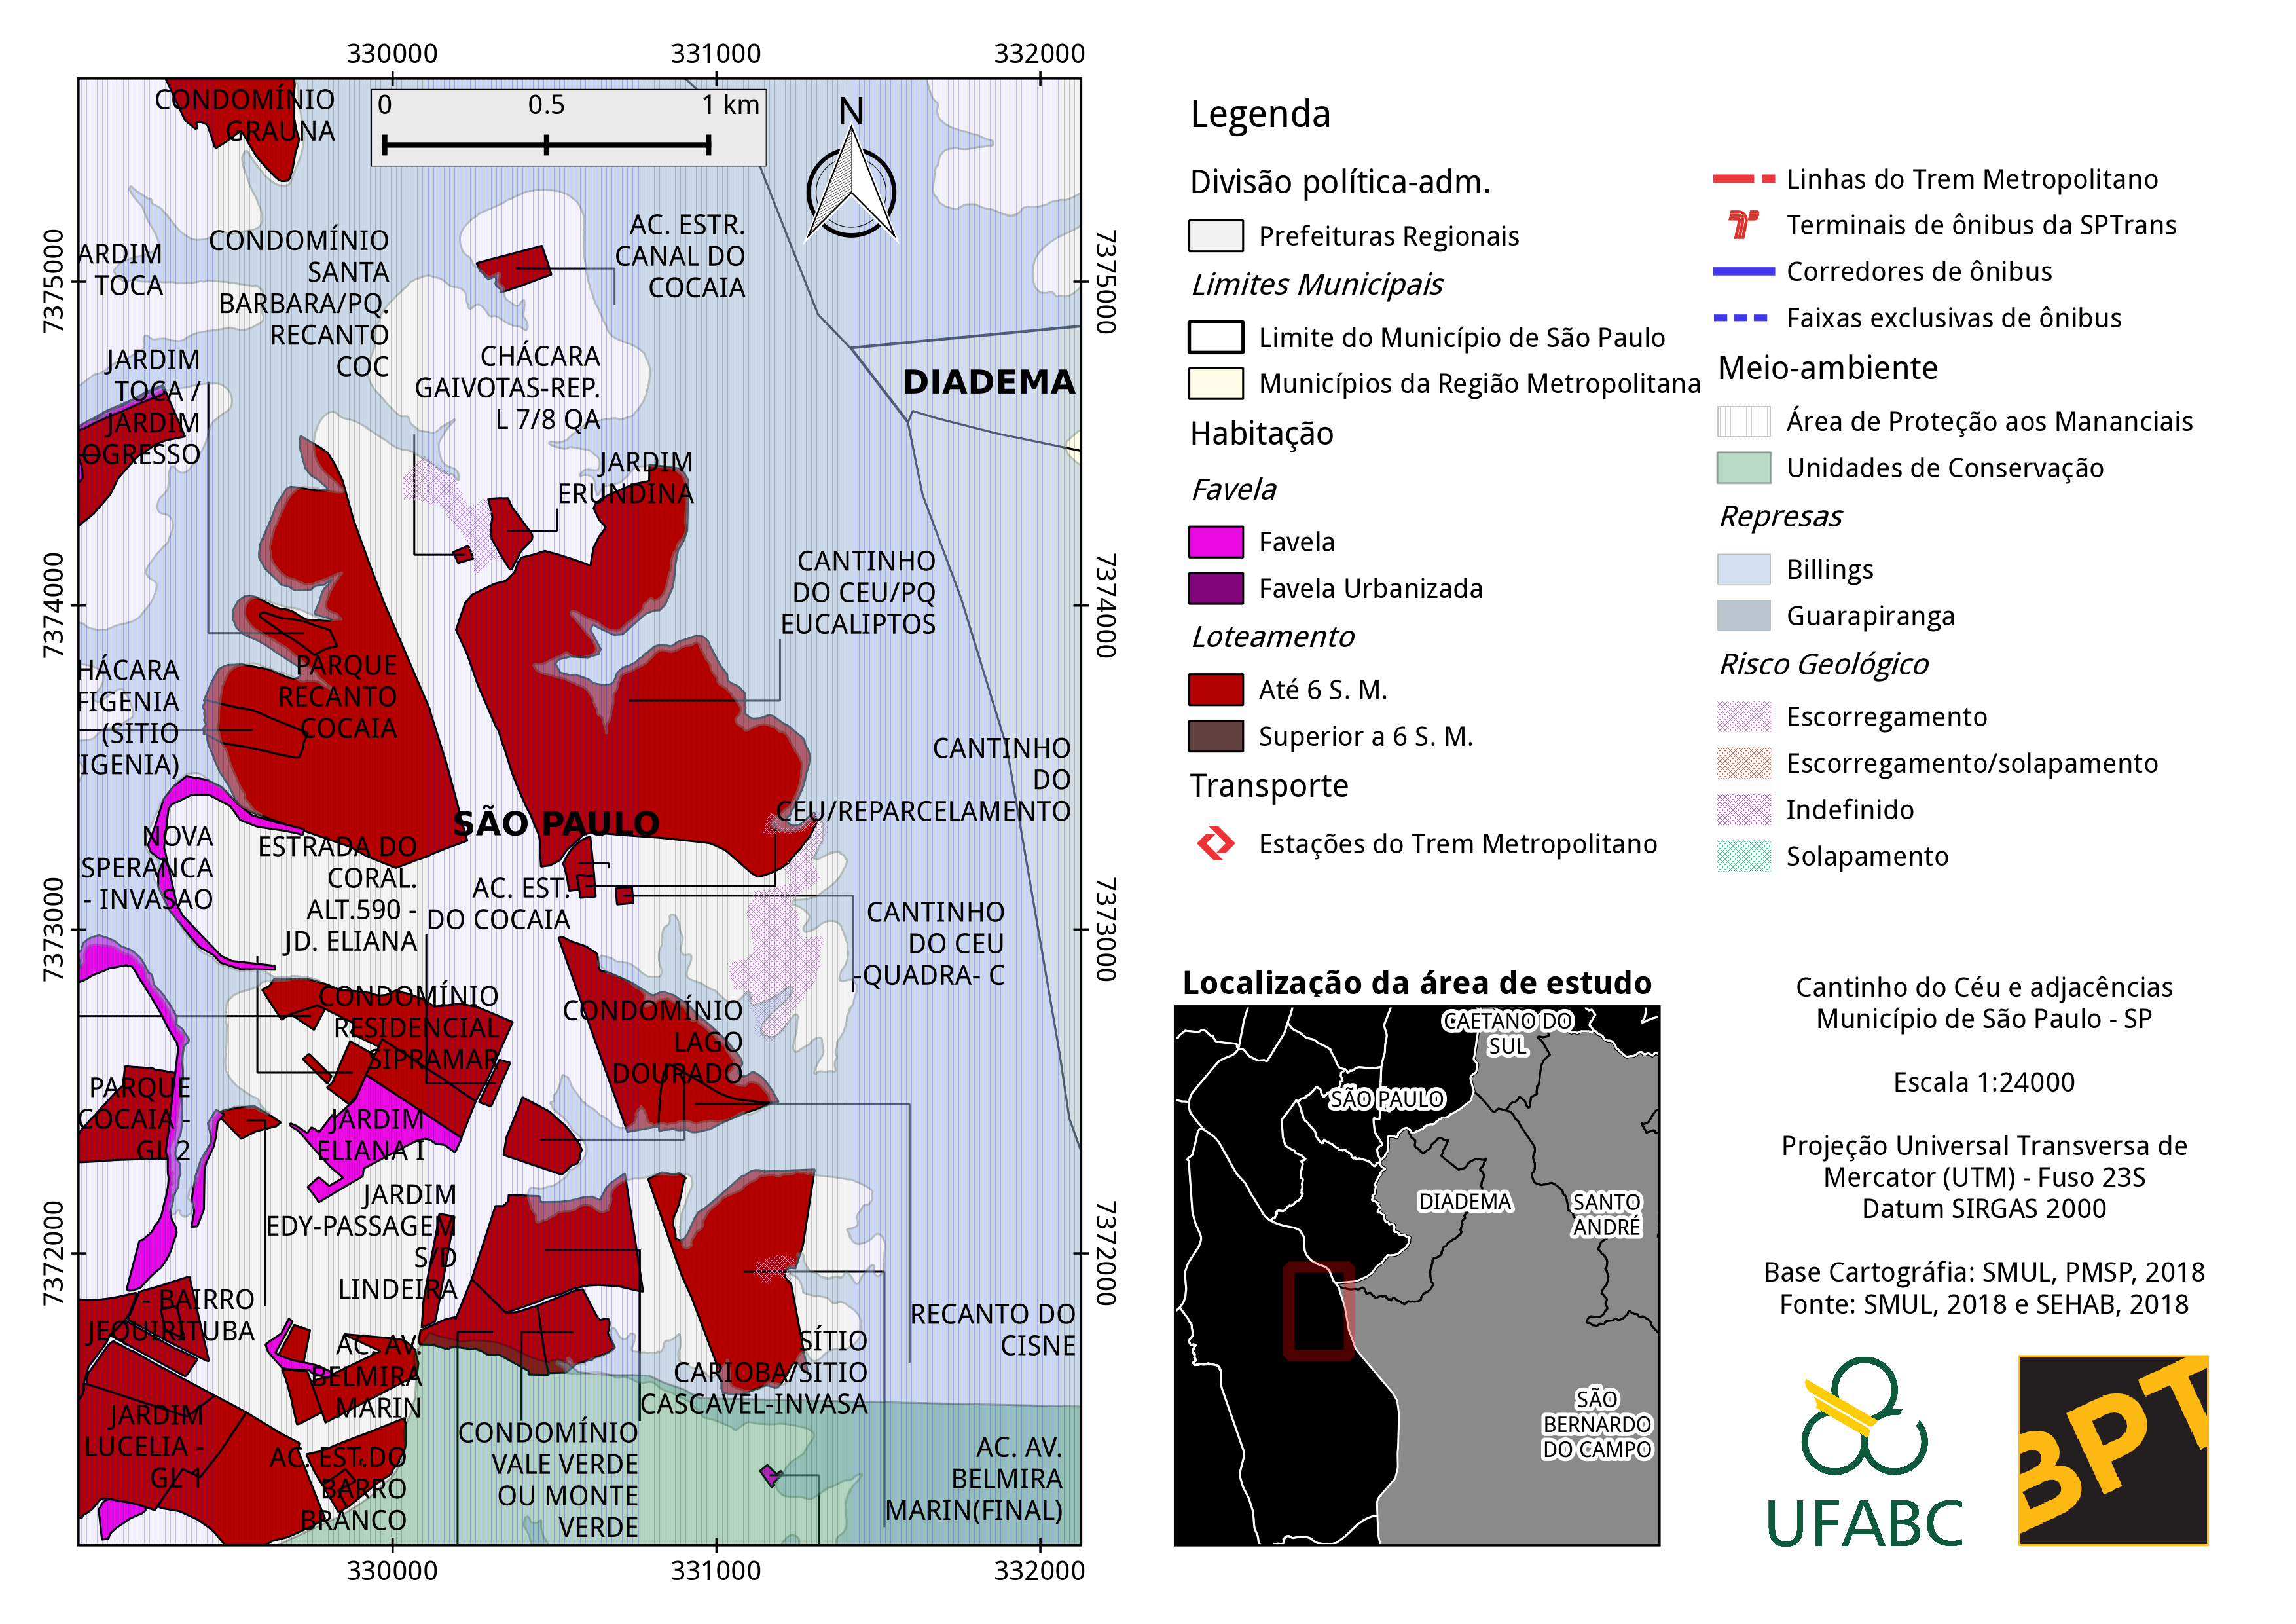
\includegraphics[height=14cm,keepaspectratio]{img/mapa_1-24000}
			\label{fig:mapa_1-24000}
			\legend{Elaboração própria}
		\end{figure}
	\end{landscape}
	
	\begin{landscape}
		\begin{figure}
			\centering
			\caption{Cantinho do Céu e Adjacências (escala 1:8400)}
			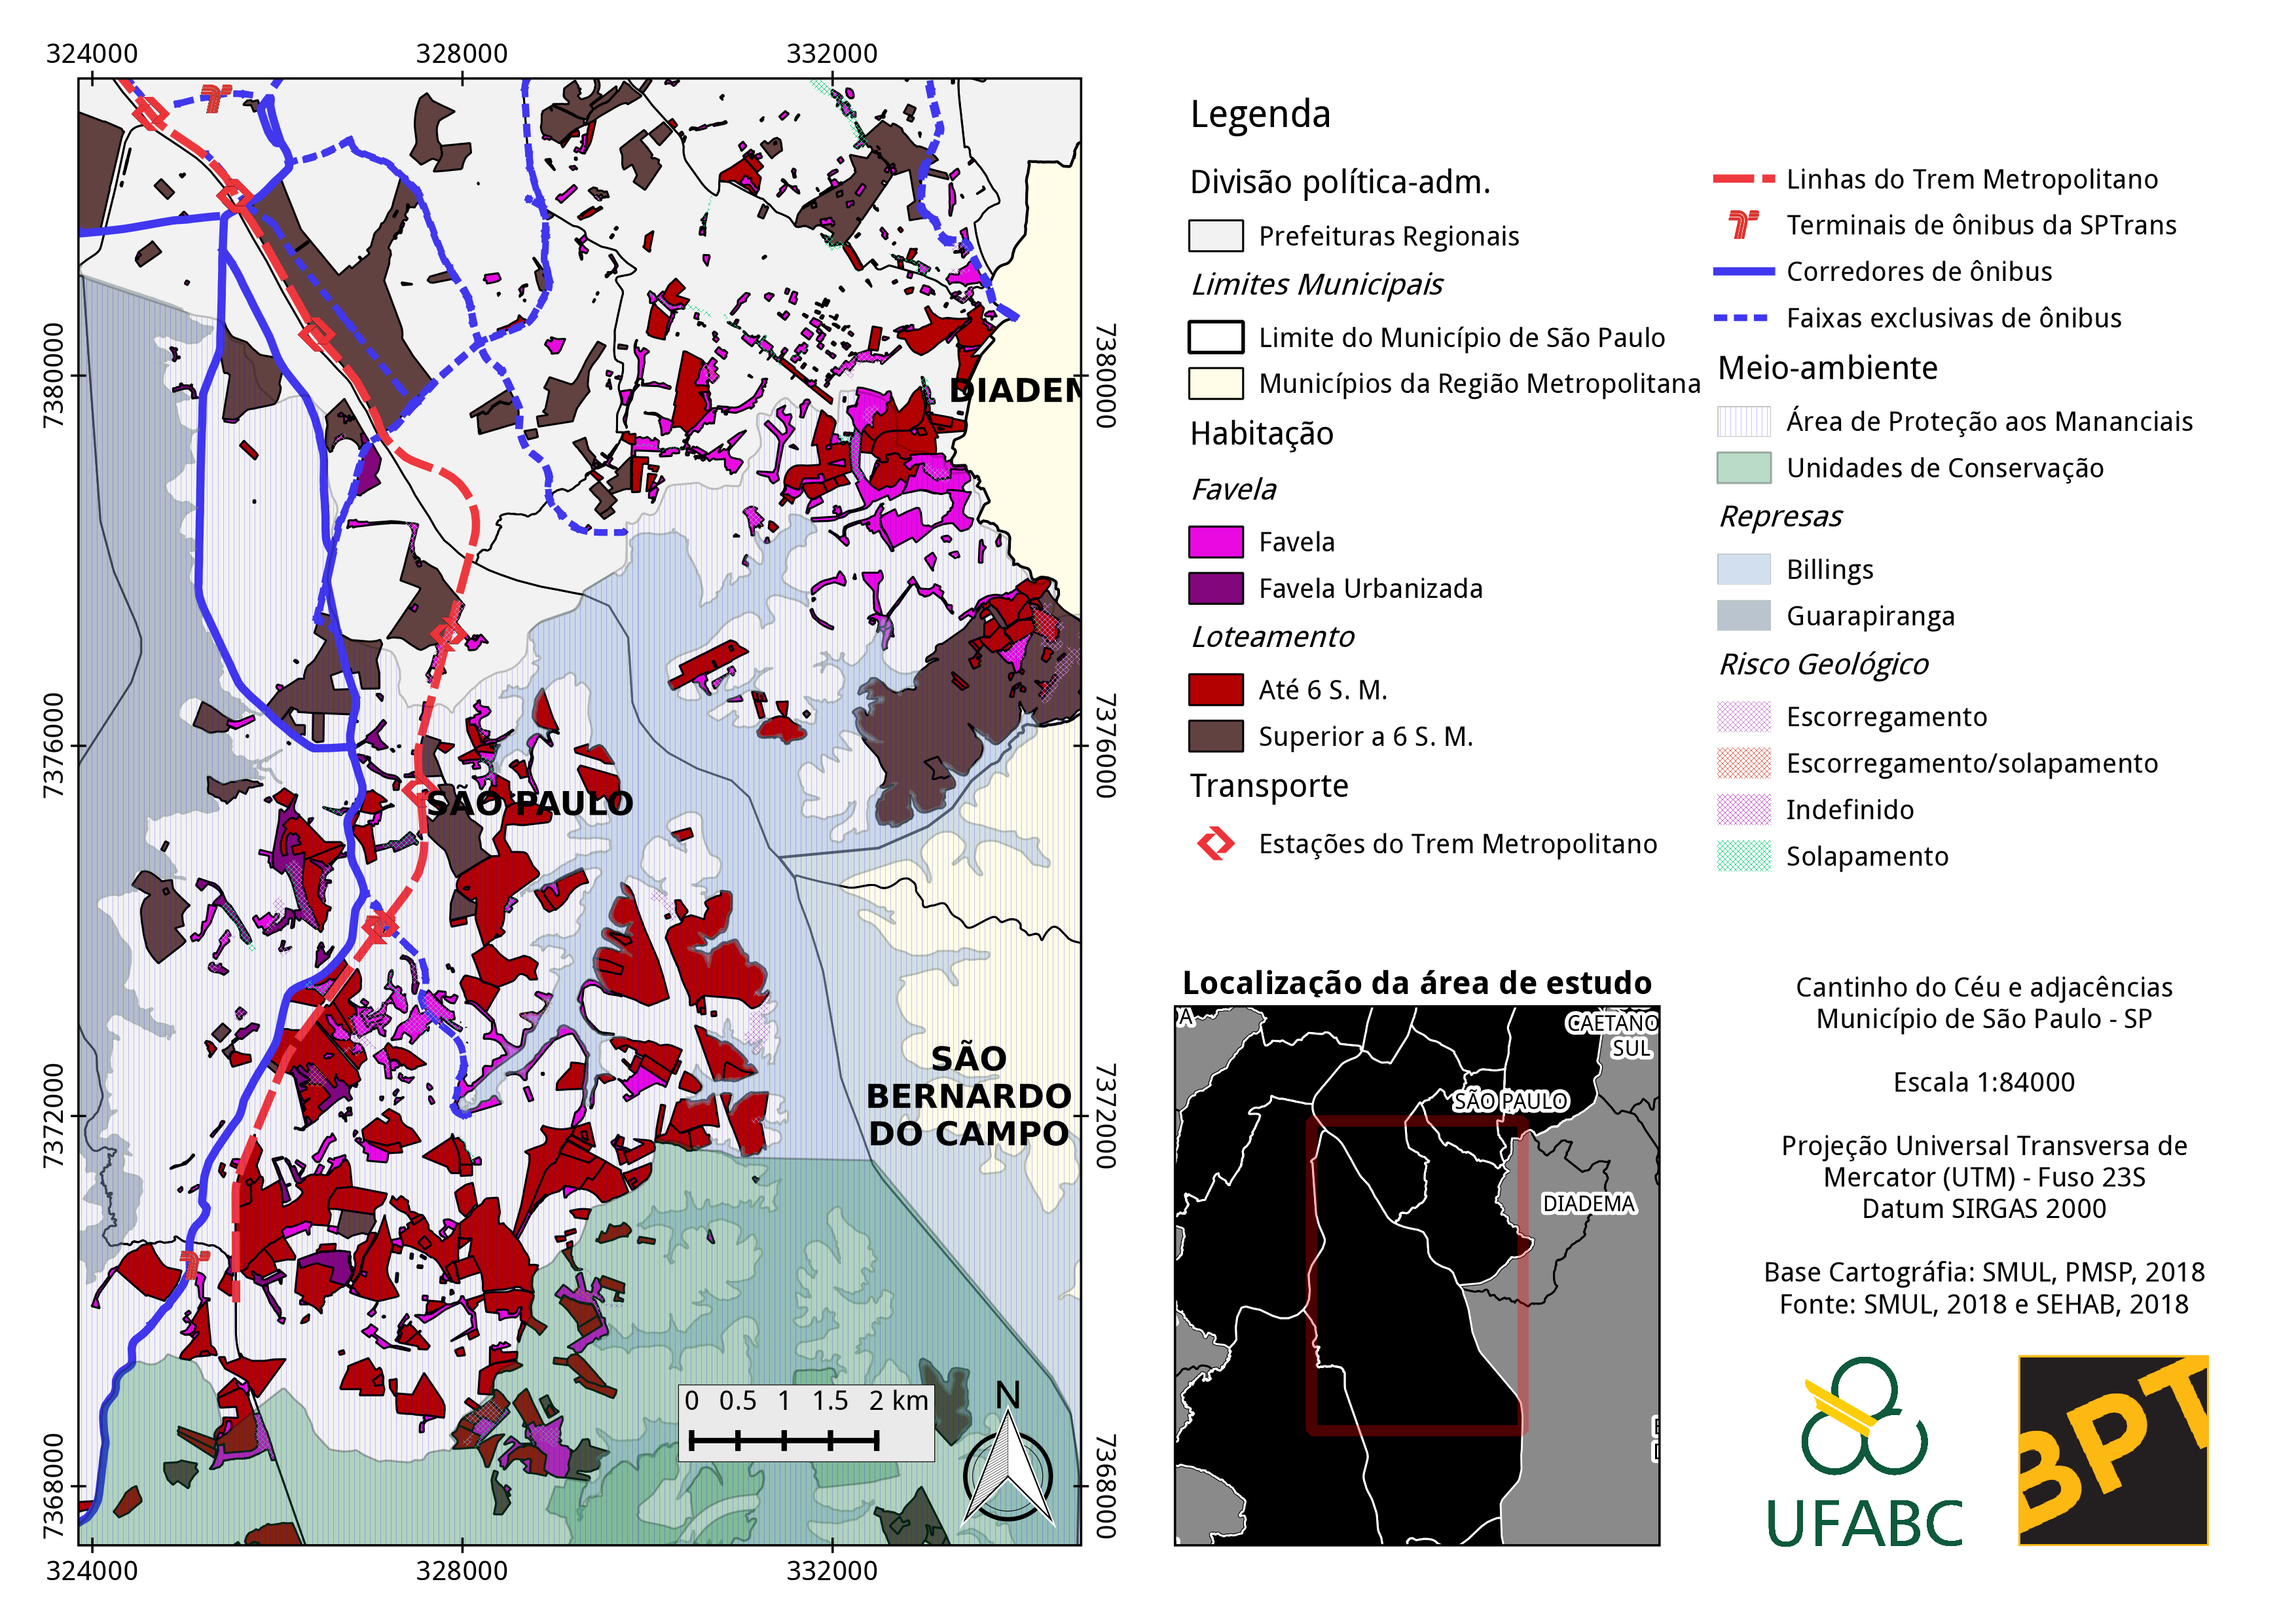
\includegraphics[height=14cm,keepaspectratio]{img/mapa_1-84000}
			\label{fig:mapa_1-84000}
			\legend{Elaboração própria}
		\end{figure}
	\end{landscape}
	
	\subsection{O processo de ocupação} \label{ocupacao}
	
	Tomando como base \citeonline[p.44-45]{Matsunaga2015}, é possível elencar as seguintes ações de relevância que precederam o surgimento da área de estudo:
	
	\begin{enumerate}
		\item 1927: a região do reservatório da represa Billings recebe o nome de Interlagos;
		\item 1932: melhoramentos viários\footnote{Vide a construção da autoestrada para Santo Amaro, denominada Autoestrada Washington Luís \cite[p.51]{Francca2000}, iniciada em 1927 e concluída em 1933, bem como uma variante desta com acesso à Cidade Satélite de Interlagos, construída em 1940 \cite[p.49]{Francca2000}} e interesses de desenvolvimento imobiliário começam a surgir junto a empreendimentos como a Riviera Paulista;
		\item 1935: até então a região pertencia ao município de Santo Amaro, passando em seguida a integrar o município de São Paulo com propósitos econômicos;
		\item 1938: parcelamento do solo no interflúvio das represas com padrões de cidade-jardim, dando origem ao Balneário Satélite Interlagos\footnote{Em \citeonline[p.51; p.56-57]{Francca2000} foi utilizado o termo Cidade Satélite Interlagos, em conformidade com o anteprojeto, bem como o termo Cidade Satélite Balneária de Interlagos, de forma que consideramos todos como sendo equivalentes e intercambiáveis};
		\item 1939: o autódromo de Interlagos começa a ser construído\footnote{Conforme \citeonline[p.51]{Francca2000} o autódromo foi financiado pela S/A Autodestradas, ligada à implantação da Cidade Satélite Interlagos, que por sua vez vende o equipamento para a Comissão organizadora dos festejos do ``IV Centenário da Cidade de São Paulo'', de maneira que o autódromo passa a ser de utilidade pública em 1951};
		\item 1940: agravamento da crise habitacional paulistana, elevando a pressão sobre os mananciais;
		\item 1959: parcelamento de habitação popular no bairro Cidade Dutra\footnote{Contíguo à Cidade Satélite de Interlagos, conforme \citeonline[p.51]{Francca2000}} em 1959, já atrelado ao polo industrial da região de Santo Amaro;
		\item 1960: marco do crescimento urbano paulistano, com a população atingindo 4 milhões de habitantes ante os 500 mil de 1920;
		\item 1960: o Iateclube Santapaula realiza adaptações no Hotel Interlagos e ali se instala \cite[p.52]{Francca2000};
		\item 1970: o poder público implanta grandes conjuntos habitacionais de interesse social nas periferias metropolitanas, contribuindo para o padrão periférico de urbanização, como o ``\gls{bnh} do Grajaú'' (Conjunto Habitacional Brigadeiro Faria Lima);
		\item 1979: a Cidade Dutra já contava com 27 mil habitantes \cite[p.51]{Francca2000}.
	\end{enumerate}
	
	Segundo \citeonline[p.80]{Silva2016}, o processo de ocupação definitiva da área de estudo se dá no final da década de 1980:
		
	\begin{citacao}
		``A ocupação da área do cantinho do Céu, assim como a do Jardim Gaivotas, dá-se em definitivo a partir de 1988, segundo documento da Associação de Moradores do Parque Residencial Cocaia Independente, logo após o surgimento de loteamento Parque dos Lagos, e Lago Azul que aconteceu em 1987 e intensificou-se nos anos 1990, em um momento de grave crise econômica e grande desemprego no país''.
	\end{citacao}

	No entanto, \citeonline{Silva2016} identificou a partir do contato com um morador local que no final dos anos 1960 a área ainda tinha características rurais \cite[p.80]{Silva2016}, situação que se alteraria nas décadas seguintes \cite[p.82]{Silva2016}:
	
	\begin{citacao}
		``Dos anos 1970-1990 a situação mais ao norte da Península do Ribeirão Cocaia ainda era pior, quanto mais ao norte mais se deterioravam as condições de vida da população, justamente onde foram implantados os bairros Cantinho do Céu e Parque Residencial Cocaia.''
	\end{citacao}
	
	\citeonline{Silva2016} também salienta que as ocupações são a maioria das moradias no bairro Cantinho do Céu, diferentemente do que acontece no Residencial Cocaia, também integrante da península do Ribeirão Cocaia \cite[p.83]{Silva2016}.
	
	Apesar da presença do transporte metroferroviário, \citeonline{Silva2016} destaca a fragilidade do Cantinho do Céu \cite[p.98]{Silva2016}:
	
	\begin{citacao}
		``Muito embora o distrito do Grajaú tenha se desenvolvido muito em algumas de suas regiões, como, por exemplo, nas áreas próximas da linha férrea Estação Grajaú da \glsdesc{cptm} (\gls{cptm}), nos bairros Jardim São Paulo, Parque América, ainda existem lugares de grande	precariedade e de espoliação urbano-ambiental, como é o caso de quase todo o bairro Cantinho do Céu e partes do próprio Grajaú (\dots)''.
	\end{citacao}
	
	Finalmente, \citeonline{Matsunaga2015} elucida a ocupação no tempo e no espaço a partir da esquematização contida na figura \ref{fig:esquema_temporal}.

	\begin{figure}[htb]
		\centering
		\caption[Esquematização temporal]{Esquematização temporal dos domínios fundiários e evolução da ocupação}
		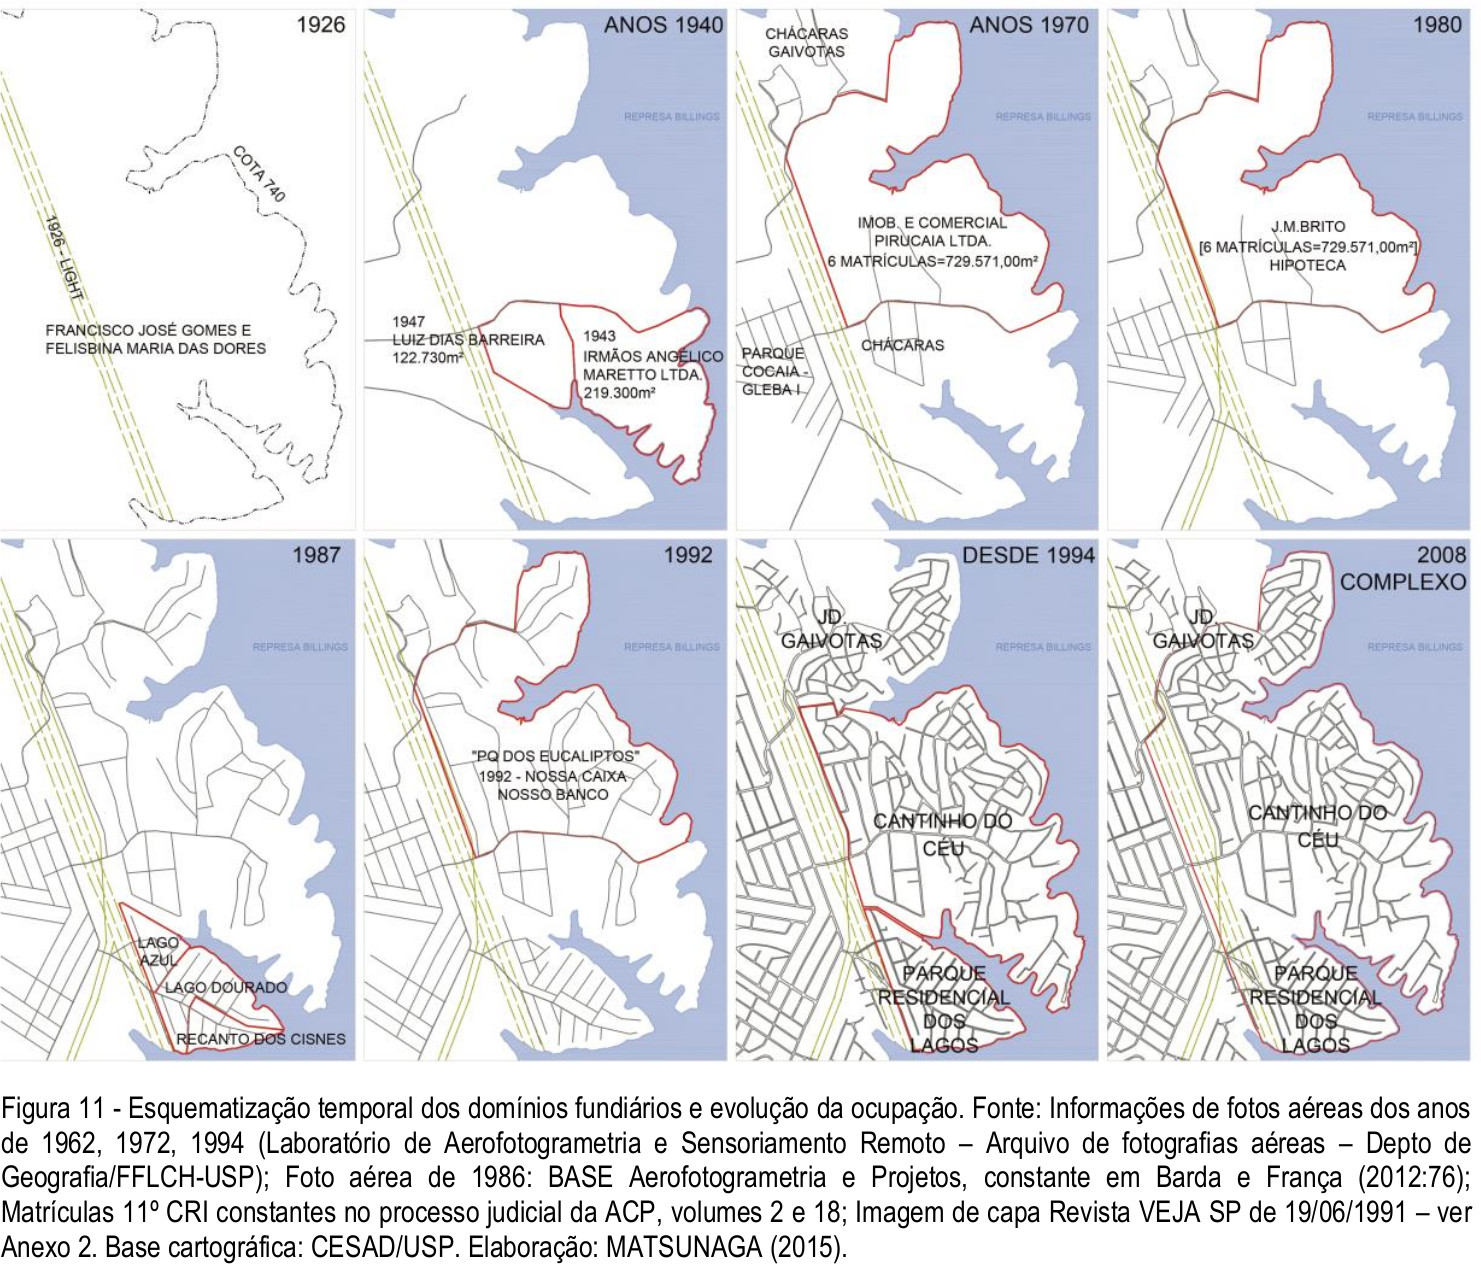
\includegraphics[width=\linewidth]{img/matsunaga_esquematizacao}
		\label{fig:esquema_temporal}
		\legend{Fonte: \citeonline[p.58]{Matsunaga2015}}
	\end{figure}
	
	\subsection{Caracterização}
	
	Conforme \citeonline[p.110]{Barda2012}, predominam no Cantinho do Céu dois tipos de ocupação: (i) parcelamento irregular e; (ii) ocupação desordenada típica de favela. Além disso, ``o tamanho médio da família do Cantinho do Céu é de 3,44 pessoas por família o que representa uma média ligeiramente superior à do município de São Paulo (3,3)'' \cite[p.110]{Barda2012}.
	
	\begin{figure}[htb]
		\centering
		\caption{Imagem aérea da área do Cantinho do Céu}
		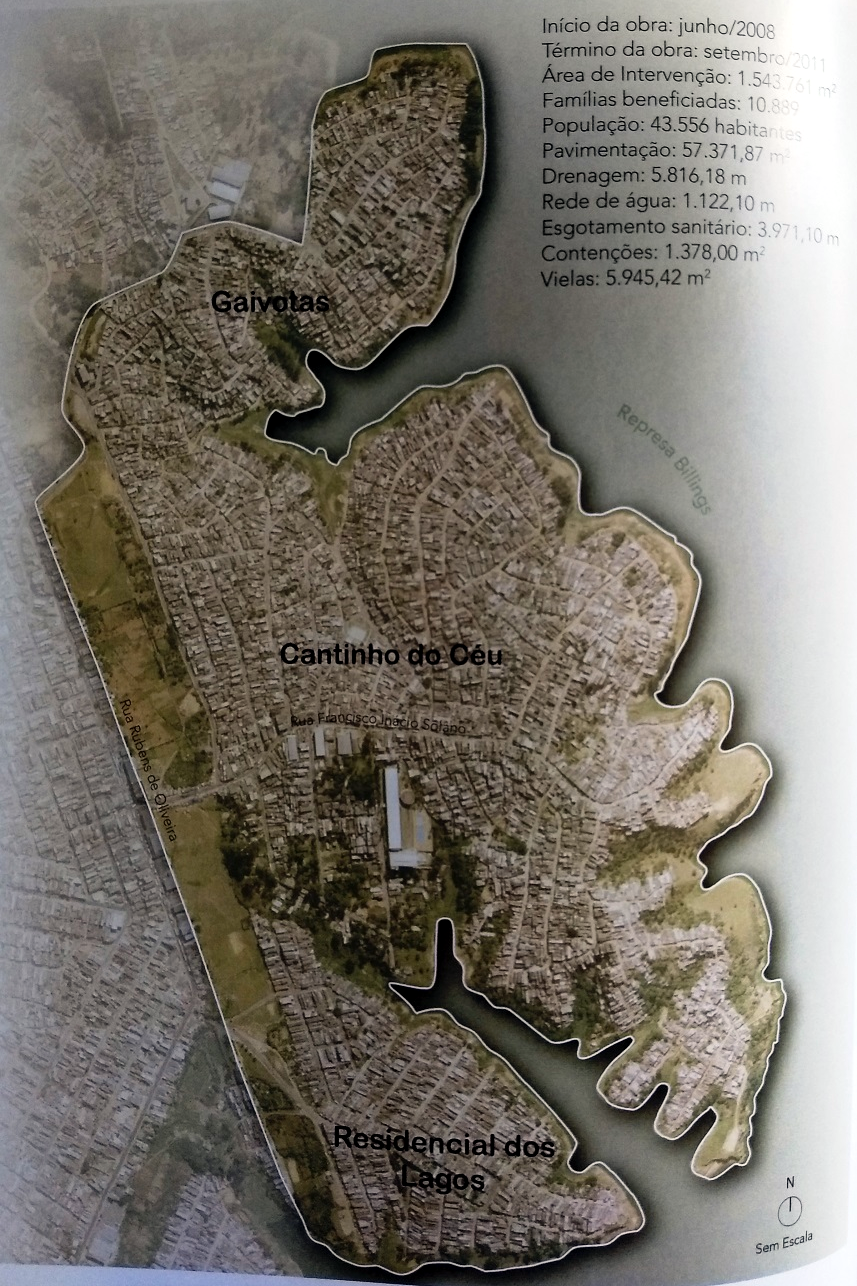
\includegraphics[height=15cm]{img/barda_peninsula}
		\label{fig:peninsula}
		\legend{Fonte: \citeonline[p.110]{Barda2012}}
	\end{figure}
	
	Os dados mostrados na figura \ref{fig:peninsula}, que mostra como está estabelecida a área do Cantinho do Céu, são reproduzidos abaixo para facilitar sua observação:
	
	% Margens ajustadas para ambiente de listas dentro do ambiente de citação conforme https://groups.google.com/forum/#!topic/abntex2/EXIZdfmYiT0
	\begin{citacao}
		\begin{itemize}[leftmargin=\leftskip+\labelwidth-\labelsep]
			\item Início da obra: junho/2008
			\item Término da obra: setembro/2011
			\item Área de intervenção: 1.543.761 m²
			\item População: 43.556 habitantes
			\item Pavimentação: 57.371,87 m²
			\item Drenagem: 5.816,18 m
			\item Rede de água: 1.122,10 m
			\item Esgotamento sanitário: 3.971,10 m
			\item Contenções: 1.378,00 m²
			\item Vielas: 5.945,42 m²
		\end{itemize}
		\cite[p.110]{Barda2012}
	\end{citacao}
	
	As figuras \ref{fig:fotos_antes_01}, \ref{fig:fotos_antes_02} e \ref{fig:fotos_antes_03} mostram o Cantinho do Céu antes do programa de urbanização. Como características marcantes, pode-se observar a proximidade de construção de algumas residências à represa, as ruas de terra e a ausência de vias que possibilitem a ligação de todas as áreas do bairro.
	
	\begin{figure}[hb]
		\centering
		\caption{Cantinho do Céu antes da urbanização}
		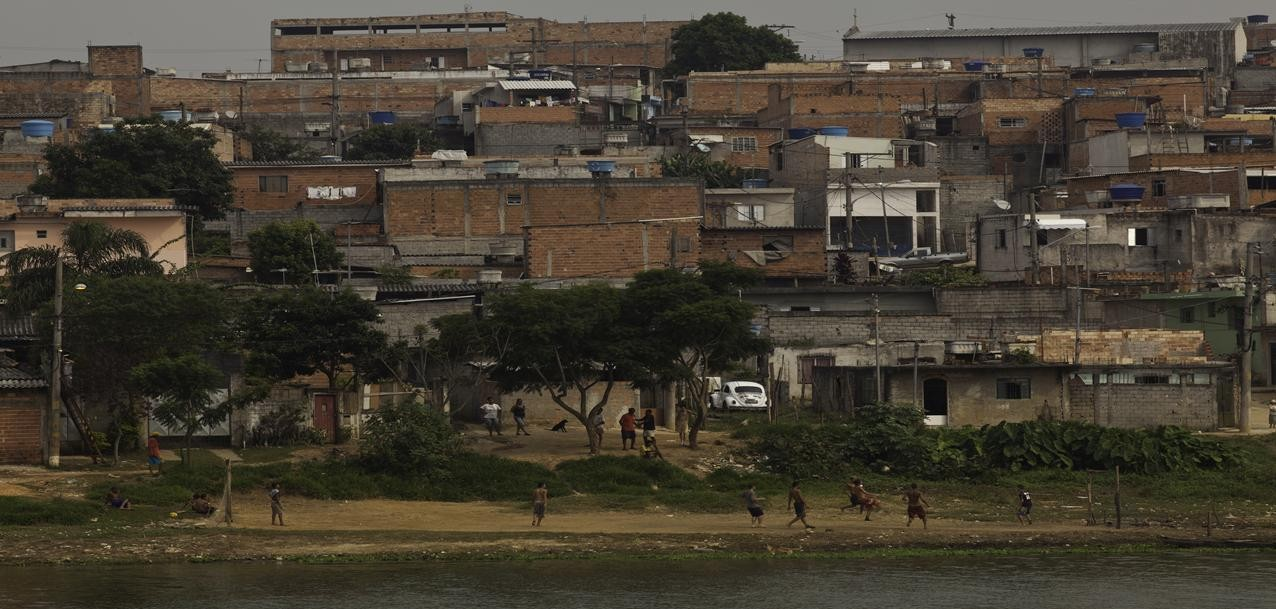
\includegraphics[width=\linewidth]{img/knoll_antes01}
		\label{fig:fotos_antes_01}
		\legend{Fonte: \citeonline{Archdaily2013}, direitos reservados a Fábio Knoll}
	\end{figure}
	
	\begin{figure}[hb]
		\centering
		\caption{Cantinho do Céu antes da urbanização}
		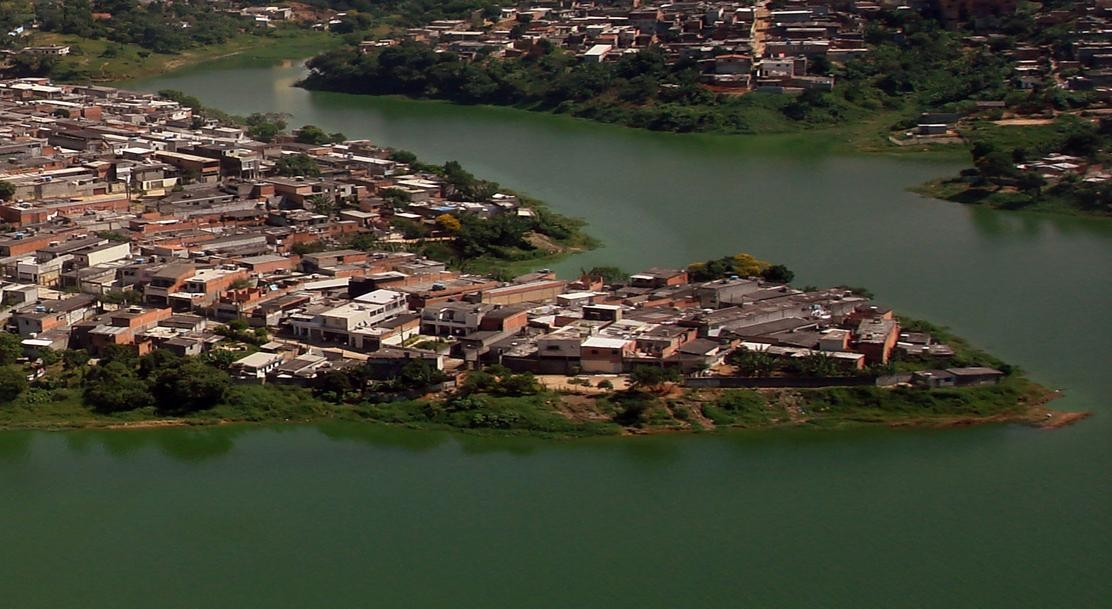
\includegraphics[width=\linewidth]{img/knoll_antes02}
		\label{fig:fotos_antes_02}
		\legend{Fonte: \citeonline{Archdaily2013}, direitos reservados a Fábio Knoll}
	\end{figure}
	
	\begin{figure}[htb]
		\centering
		\caption{Cantinho do Céu antes da urbanização}
		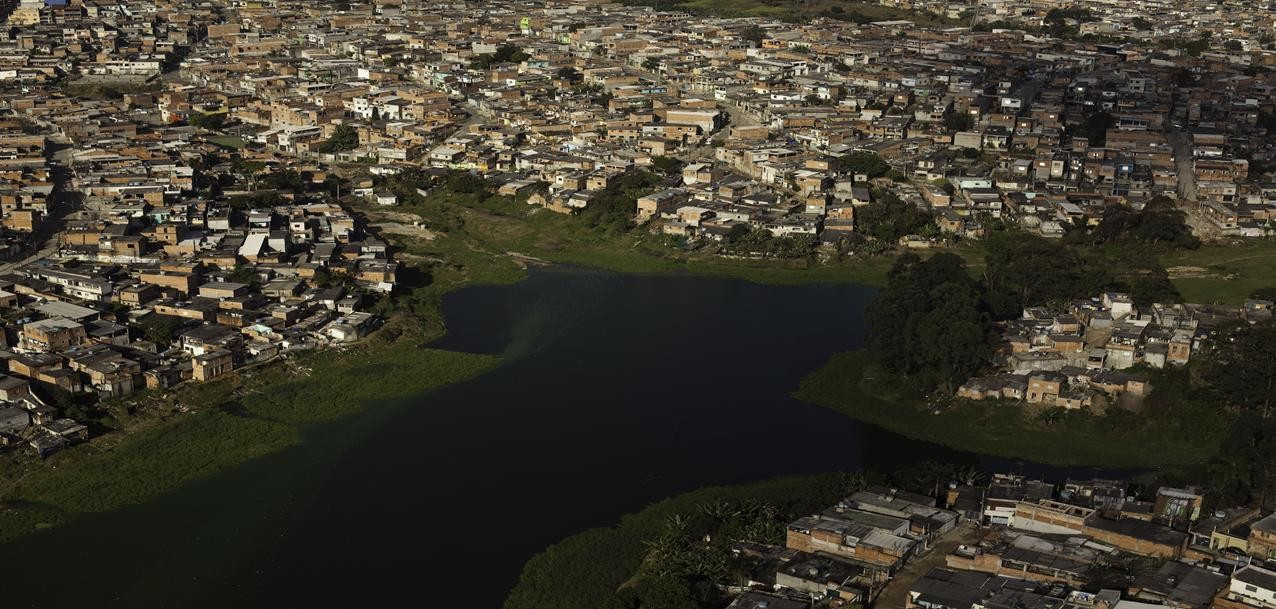
\includegraphics[width=\linewidth]{img/knoll_antes03}
		\label{fig:fotos_antes_03}
		\legend{Fonte: \citeonline{Archdaily2013}, direitos reservados a Fábio Knoll}
	\end{figure}
	
	\chapter{Projeto de intervenção}
	
	Como vimos nas subseções \ref{light} e \ref{ocupacao}, ainda que sumarizados e resumidos, os desdobramentos que levaram à ocupação e posterior urbanização do Cantinho do Céu foram muitos, no entanto, como ponto de partida para entendimento das ações de urbanização, pode ser citado o Programa Guarapiranga, que foi iniciado em 1990, devido à realidade da ocupação irregular das áreas de mananciais, bem como ao agravamento da qualidade das águas do reservatório. O programa foi constituído por um conjunto de intervenções de infraestrutura, sumarizadas na figura \ref*{tab:francca_programa}. Podemos compreender a seguir a justificativa para o programa, conforme \citeonline[p.27-28]{Francca2000}:
	
	\begin{citacao}
		``No período 1977/89, a qualidade da água do reservatório piorava, ameaçando o abastecimento público proporcionado pelo Sistema Guarapiranga; neste particular os anos de 1990 e 1991 foram críticos. Diante desta situação e a partir da experiência integrada das ações de fiscalização do SOS Mananciais, iniciou-se, em 1991, a preparação de um programa de atividades que tinha como objetivo central a recuperação da qualidade das águas do manancial para o abastecimento público. Os trabalhos iniciais foram conduzidos pela \gls{sabesp} -- \glsdesc{sabesp}, com participação da então Secretaria Nacional de Saneamento do Ministério da Ação Social, hoje extintos, e com o apoio do \glsdesc{bird} -- \gls{bird}, dentro de um programa de ações mais amplo, que envolvia as regiões metropolitanas de Belo Horizonte e Curitiba.''
	\end{citacao}
	
	\begin{table}[htb]
		\centering
		\caption{Programa de Saneamento Ambiental da Bacia do Guarapiranga}
		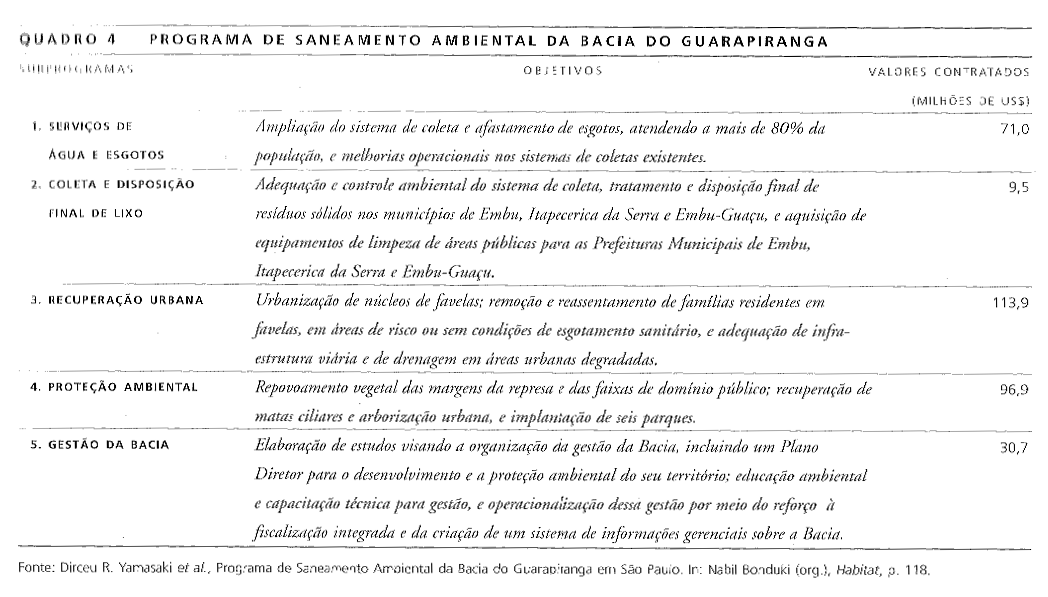
\includegraphics[width=\linewidth]{img/francca_p029_tabela_programa}
		\label{tab:francca_programa}
		\legend{Extraído de: \citeonline[p.29]{Francca2000}}
	\end{table}
	
	\citeonline[p.21]{Barda2012} oportunamente recupera o papel do Programa Guarapiranga e o relaciona com a situação da região da represa Billings e os desdobramentos posteriores, no âmbito do Programa Billings Legal:
	
	\begin{citacao}
		``No ano de 1997, teve início a terceira etapa da primeira fase do Programa Guarapiranga, mesmo ano em que era aprovada a nova legislação de proteção dos mananciais (Lei Estadual 9.866/97), a qual estabelecia o Plano Emergencial, permitindo que os órgão públicos, como a Sabesp e as prefeituras implantassem ações de saneamento básico na região dos mananciais sul, desde que os bairros fizessem parte da lista de áreas precárias publicadas como parte integrante da legislação.
		
		O Plano Emergencial produziu rápida manifestação de lideranças da região Billings, exigindo que as ações do programa de urbanização se estendessem para seus bairros. Duas das lideranças mais ativas eram do Cantinho do Céu (Floripes) e do Jardim Gaivotas (Emília), que participavam ativamente das reuniões do subcomitê da bacia Billings.
		
		Como resposta às demandas da população por soluções para atenuar as condições precárias dos bairros irregulares da região, a \gls{sehab} preparou o Programa Billings Legal, buscando recursos financeiros para sua execução e a integração das ações com o Governo do Estado.''
	\end{citacao}

	Ainda segundo \citeonline[p.21]{Barda2012}, no diagnóstico elaborado em função do programa, ficou claro que a área do Cantinho do Céu era uma das mais carentes da cidade de São Paulo e tinha como condição crítica seu esgotamento sanitário, que ``era efetuado por meio de fossas negras, sujeitas a extravasões frequentes para as valas de drenagem irregulares de águas pluviais''.
	
	Quanto aos desdobramentos do Programa Billings Legal, \citeonline[p.21]{Barda2012} faz a seguinte descrição\footnote{Para breves detalhes sobre os antecedentes do Programa Mananciais, ver \citeonline[p.51]{Matsunaga2015}}:
	
	\begin{citacao}
		``Em 2005 foi retomado com o nome de Programa Mananciais, inicialmente uma parceria entre os governos municipal e estadual e, a partir de 2010, com recursos do governo federal.
		
		Nesse momento, a \gls{sehab} deu início à elaboração do novo projeto para o Cantinho do Céu, em parceria com a equipe técnica do Ministério Público, com o propósito de encontrar soluções de consenso que permitissem a permanência da maioria das famílias no local. Ao mesmo tempo se buscava a recuperação ambiental da região da península, através da implantação das redes de coleta de esgoto, sistemas de drenagem, eliminação de áreas de risco e implantação de espaços públicos.''
	\end{citacao}
	
	O projeto de urbanização da área do Cantinho do Céu se inicia no ano de 2008, com duração de quatro anos e término no final de 2012. Apenas após o processo de contratação das obras, em 2010 (dez anos depois dos primeiros estudos), o canteiro de obras e as máquinas se instalaram no Cantinho do Céu \cite{Barda2012}. Identificamos que a decisão de urbanizar surgiu como alternativa à remoção em massa das famílias, ou seja, a opção pela urbanização teve origem na frustração da ação originalmente prevista em 2002, quando a \gls{sehab} recebeu uma ordem do Ministério Público para readequar urbanisticamente a região, com sua desocupação em 30 dias, o que se mostrou inviável devido aos cerca de 20 mil habitantes que precisariam ser removidos, o que deu início a diálogos junto ao Ministério Público para o desenvolvimento de outras alternativas que pudessem solucionar do problema habitacional da região. \cite[p.21]{Barda2012}
	
	Conforme \citeonline[p.116]{Barda2012}, ``a partir de 2005, começamos a trabalhar e idealizamos um plano conjunto com vistas a manter a população que ali vivia, dotando a área da estrutura necessária''; em 2008 o escritório de Arquitetura  Boldarini Arquitetura e Urbanismo inicia as obras de intervenção sobre a região.

	Eventos-chave, como os que abriram este capítulo, bem como outros elencados no capítulo \ref{light}, encontram-se sumarizados na figura \ref*{fig:cronologia}. Adicionalmente, uma consolidação mais abrangente, incluindo aspectos ligados ao marco regulatório e formatação institucional foi elaborado por \citeonline{Matsunaga2015} em uma linha do tempo que visa ``elucidar o processo nas diversas escalas'' \cite[p.37]{Matsunaga2015}, conforme podemos ver na figura \ref*{fig:matsunaga_linha}.
	
	\begin{figure}[htb]
		\centering
		\caption[Cronologia do surgimento do Cantinho do Céu]{Breve diagrama de eventos cronológicos que desencadearam no surgimento do Cantinho do Céu}
		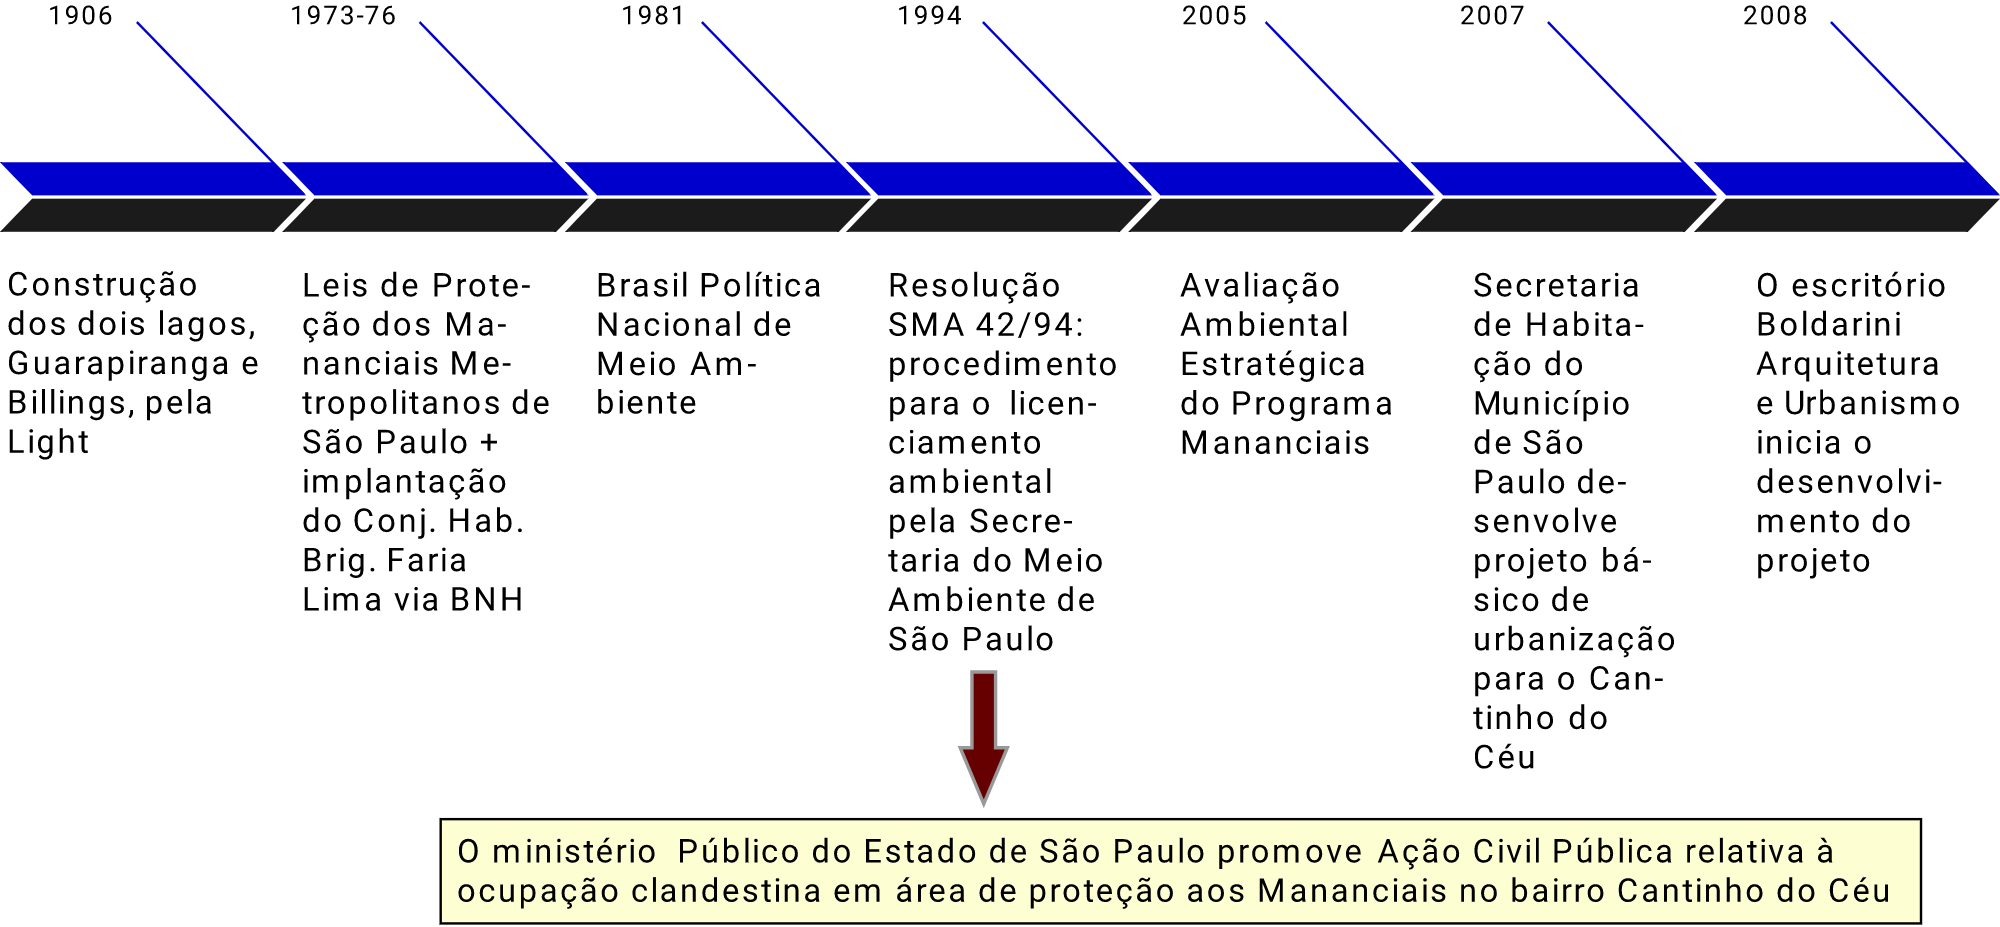
\includegraphics[height=7cm]{img/cronologia}
		\label{fig:cronologia}
		\legend{Elaboração própria com base em \citeonline{Barda2012}}
	\end{figure}
	
	\section{Objetivo do projeto}
	
	O objetivo do projeto era propor uma urbanização adequada sobre toda a região do Lago Azul, dotando-o de toda a infraestrutura necessária, permitindo o desenvolvimento de sua população como indivíduo e sociedade. Dentre todas as ações necessárias, pode-se citar algumas ações tomadas como estratégias de intervenção, sendo elas \cite{Archdaily2013} \cite[p.28]{Barda2012}:
	
	\begin{itemize}
	    \item Preservação da vida, realizando correções em todas as áreas/habitações identificadas que apresentavam risco a segurança e saúde da população;
	    \item Integração urbanística entre as novas intervenções, permitindo o acesso as demais áreas, respeitando a tipologia de cada região;
	    \item Correção na infraestrutura urbana, adequando e implementando redes de esgoto, realizando melhorias ambientais e ampliação da malha rodoviária ;
	    \item Geração de condições para a realização da regularização fundiária de todos os integrantes da região.
	\end{itemize}
	
	Conforme \citeonline{Archdaily2013} e \citeonline[p.28]{Barda2012}: ``a qualificação urbana e ambiental do Cantinho do Céu, a que se propõe o projeto de urbanização, se materializa no  `tudo ao mesmo tempo', em que as ações ocorrem de forma simultânea, orquestradas pelo eixo da criação dos espaços públicos''. Sendo as intervenções esquematizadas conforme figura \ref{fig:proposta_arq}\footnote{Diagrama similar também está presente em \citeonline[p.27]{Barda2012}}.
	
	\begin{figure}[htb]
		\centering
		\caption{Diagramas do projeto urbanístico}
		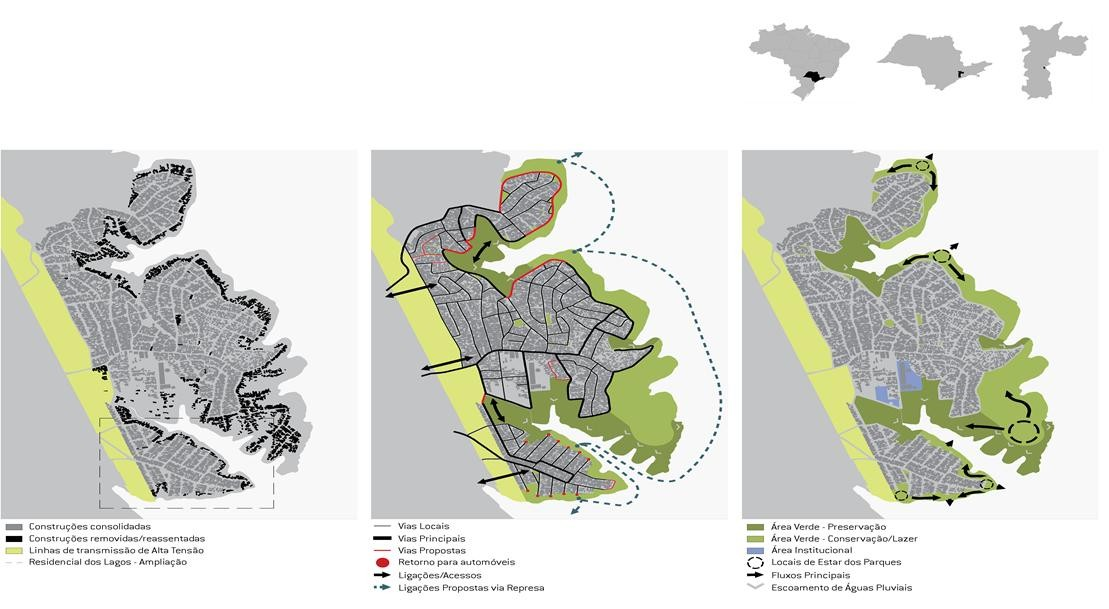
\includegraphics[width=\linewidth]{img/proposta}
		\label{fig:proposta_arq}
		\legend{Fonte: \citeonline{Archdaily2013}}
	\end{figure}
	
	\section{Dificuldades encontradas}
	
	Como todo o projeto de intervenção e adequação de favelas, o projeto do Cantinho do Céu também apresentou dificuldade de concepção durante todo o período de implementação.
	
	A primeira dificuldade apresentou-se quanto a recepção da própria população do local. Em primeiro momento a população mostrava certa resistência frente ao programa, alegando que não era primeira promessa de melhoria do local e que, como a anterior, também não seria cumprida conforme prometido. Porém, com o avanço do projeto e as melhorias ganhando destaque na região, a população passa a aceitar mais ao programa e a interagir mais com as equipes, aumentando a aproximação entre as partes.
	
	Quanto à região, o projeto enfrentou dificuldade a respeito de sua topologia devido a sua declividade acentuada e a desordenada implementação que ocorrera no bairro ao longo dos anos. Estes fatores dificultaram o processo de implementação das redes de esgoto e da malha viária. Para a realização desta atividade foi necessário que cerca de 10\% das famílias fossem removidas para outras regiões, permitindo o acesso e início de obras. 
	
	Ressalta-se ainda dificuldade frente aos órgãos públicos para a concepção do projeto. Para a realização da intervenção, se fez necessário integração da Secretaria do Verde e Meio Ambiente, das secretarias da Educação e Saúde; do Governo do Estado participaram a Secretaria de Saneamento, Secretaria de Meio Ambiente e Sabesp. Segundo Ricardo Sampaio, engenheiro integrante da equipe de intervenção, realizar o trabalho integrado entre todos os órgãos e secretarias atuantes sobre o projeto mostrou-se como um dos maiores desafios enfrentados pela equipe \cite[p.121]{Barda2012}.
	
	Finalmente, \citeonline[p.93]{Silva2016} faz uma crítica ao projeto engendrado pelo poder público, citando as remoções e considerando que não foi fornecida uma solução clara para o problema da habitação, além de destacar a assimetria ligada à apropriação do lugar, com nomes díspares entre população e poder público, elemento este que inclusive provocou confusão quando da realização deste relatório:
	
	\begin{citacao}
		``E, ainda, temos de lembrar que houve remoções de população nesse período para a construção do parque linear que a Prefeitura chama de Cantinho do Céu, e os moradores chamam de Lago Azul, e operações de desfazimento durante a administração Kassab (2006-2008), quando	assumiu a prefeitura substituindo José Serra (2009-2012), que removeu pessoas das áreas de mananciais sem proporcionar uma solução clara para o problema da habitação (\dots)''
	\end{citacao}
	
	Conforme a figura \ref{fig:lago_cantinho}, as áreas do Lago Azul e Cantinho do Céu ficam bastante próximas, ainda que o reservatório exerça um obstáculo, que teria sido superado caso o projeto tivesse sido implantado em sua totalidade (aspecto este aprofundado no capítulo \ref{hoje}).
	
	\begin{figure}[htb]
		\centering
		\caption[Lago Azul e Cantinho do Céu em 30/05/2015]{À direita, o Lago Azul e, à esquerda, vista do Cantinho do Céu; no centro da foto, área do reservatório Billings, 30 de maio de 2015}
		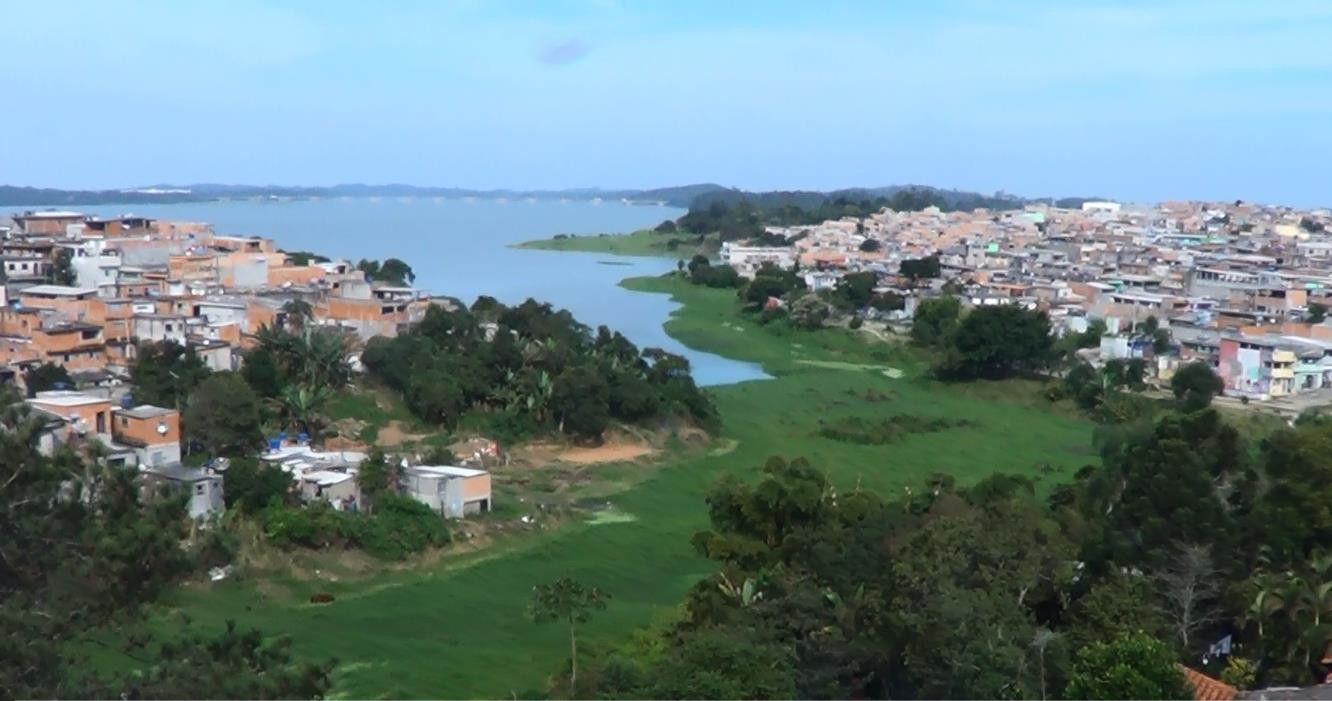
\includegraphics[width=\linewidth]{img/silva_p080_lago_cantinho}
		\label{fig:lago_cantinho}
		\legend{Fonte: \citeonline[p.80]{Silva2016}}
	\end{figure}
	
	\section{Algumas soluções adotadas}

	Para implementação do projeto algumas medidas tiveram de ser adotadas para atender toda a demanda que era necessária e, simultaneamente, tornar o projeto viável.
	
	Devido as dificuldades apresentadas durante a elaboração do escopo de intervenção, tais como a dificuldade de uma pré-concepção de projeto devido a falta de conhecimento prévio da região e resistência da população frente ao projeto, foi desenvolvida uma metodologia para implementação em etapas concomitantes, ou seja, esta ocorreria de forma gradual e seletiva, separando em etapas e partes todas as áreas de atuação. As figuras \ref{fig:barda_etapas} e \ref{fig:barda_trecho_reslagos} ilustram tal abordagem.
	
	Esta medida favoreceu, principalmente, no aceite por parte da população, que foi capaz de visualizar a evolução gradual do processo e também participar de toda a estruturação que estava ocorrendo em sua região. Além deste fato, esta medida possibilitou a equipe de desenvolver e implementar tecnologias específicas em cada região, como por exemplo o asfalto que cobria as rodovias. Como cada região apresentava um tipo de tipologia, inclinação e estrutura do solo, cada região apresentava um tipo de asfalto que melhor se adaptava a estas condições. Para um exemplo de soluções adotadas numa das ruas do Parque Residencial dos Lagos, consulte a figura \ref{fig:solucoes}.

	\noindent
	\begin{minipage}[b]{.53\textwidth}
		\captionof{figure}{Cantinho do Céu -- divisão de obras em etapas}
		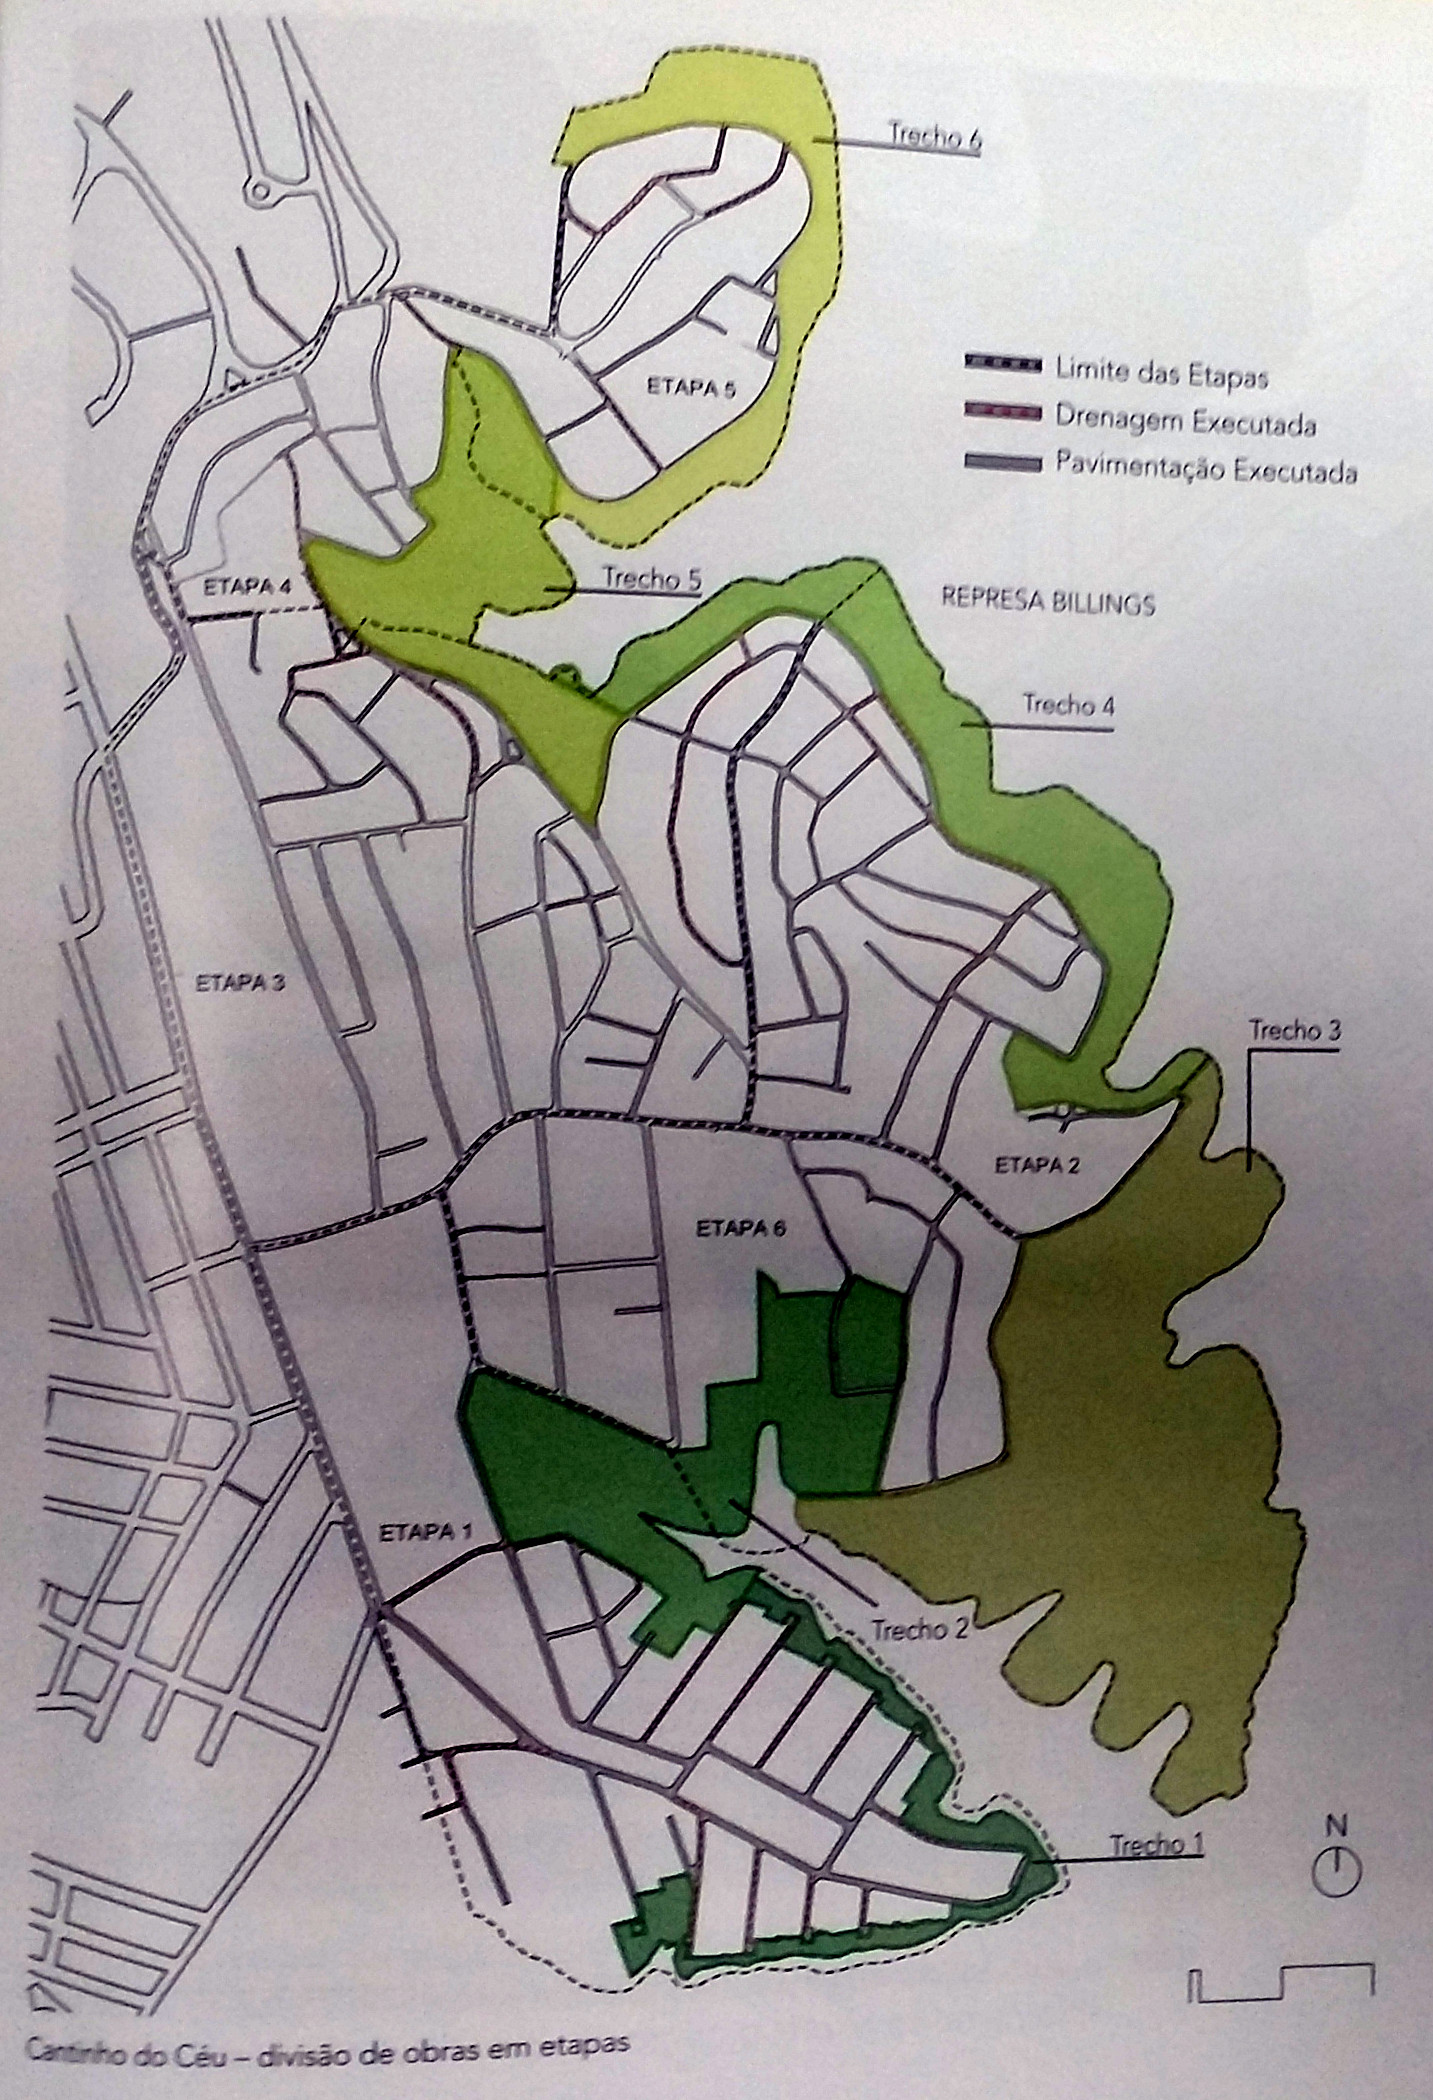
\includegraphics[width=\linewidth]{img/barda_etapas}
		\label{fig:barda_etapas}
		\legend{Fonte: \citeonline[p.117]{Barda2012}}
	\end{minipage}%
	\hfill
	\begin{minipage}[b]{.4\linewidth}
		\captionof{figure}{Residencial dos Lagos -- divisão das obras em partes}
		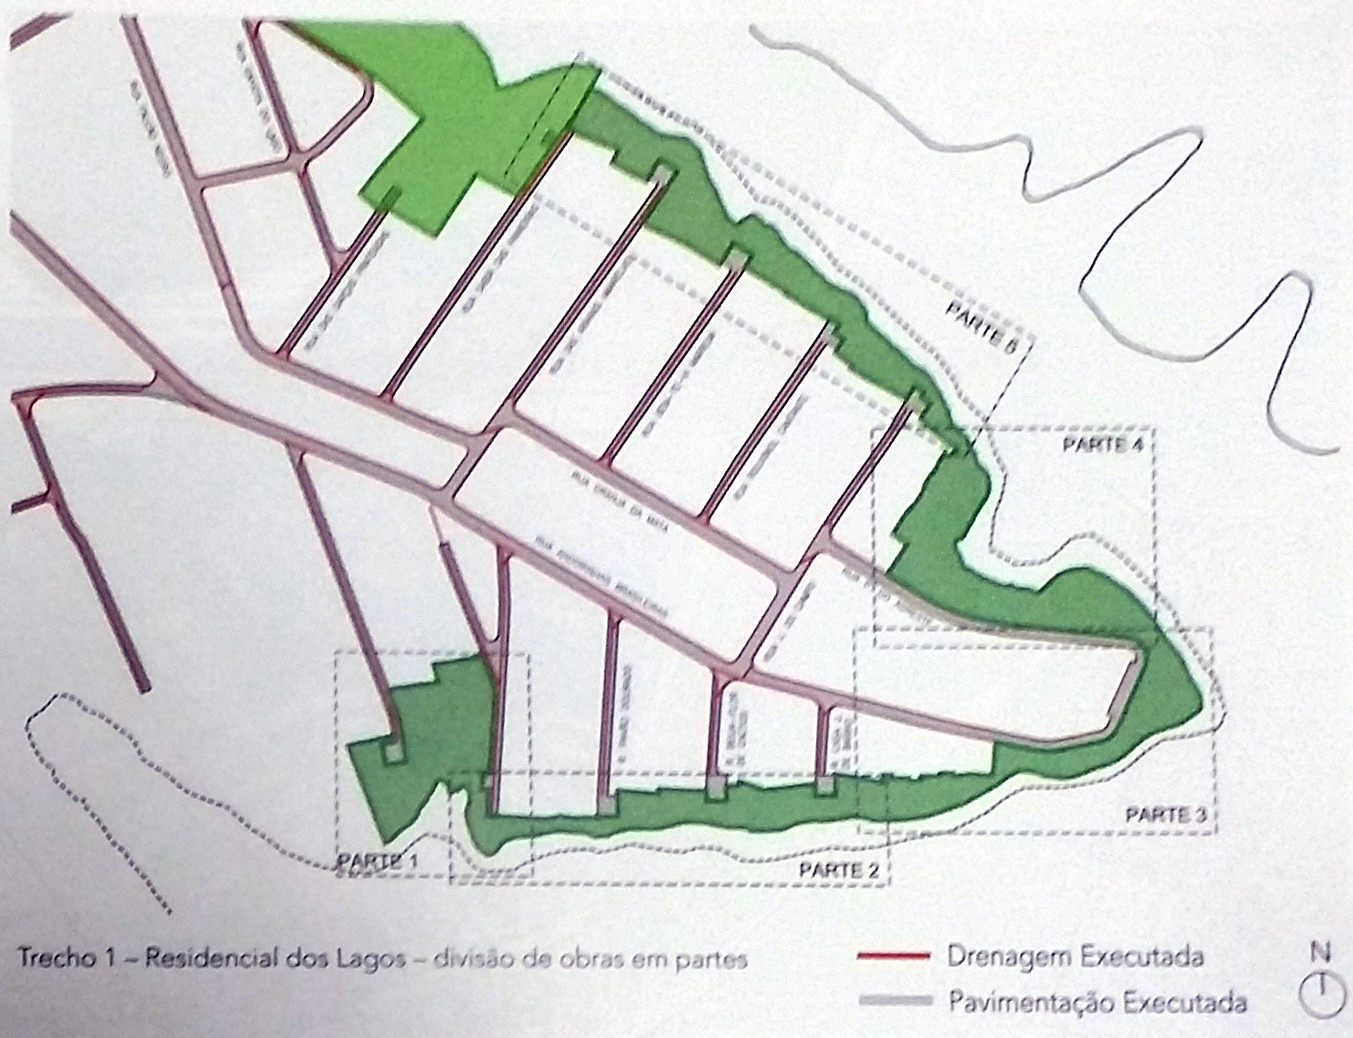
\includegraphics[width=\textwidth]{img/barda_trecho_reslagos}
		\label{fig:barda_trecho_reslagos}
		\legend{Fonte: \citeonline[p.117]{Barda2012}}
	\end{minipage}
	
	Por fim, executar o projeto em etapas permitiu a tomada de soluções em questão do cronograma financeiro e as aprovações do projeto. A solução adotada pela equipe foi atuar e ajustar o cronograma financeiro conforme as etapas eram aprovadas pelos órgãos públicos \cite{Barda2012}.
	
	\begin{figure}[htb]
		\centering
		\caption[Soluções adotadas na rua Casa do João de Barro]{Rua Casa do João de Barro: solução tipo de infraestrutura e sistema tipo de drenagem, julho de 2008}
		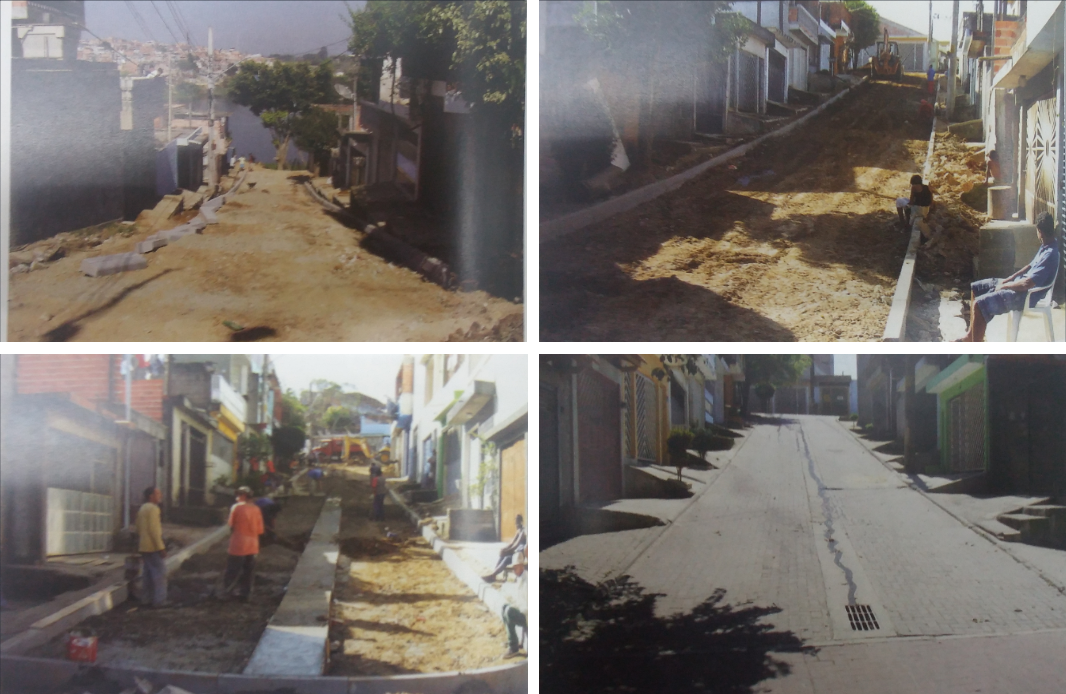
\includegraphics[width=\linewidth]{img/barda_solucoes}
		\label{fig:solucoes}
		\legend{Fonte: \citeonline[p.120]{Barda2012}}
	\end{figure}
	
	% ------------------------------------------------------------
	% Manter aqui, antes do próximo capítulo
	\begin{landscape}
		\begin{figure}
			\centering
			\caption{Linha do tempo}
			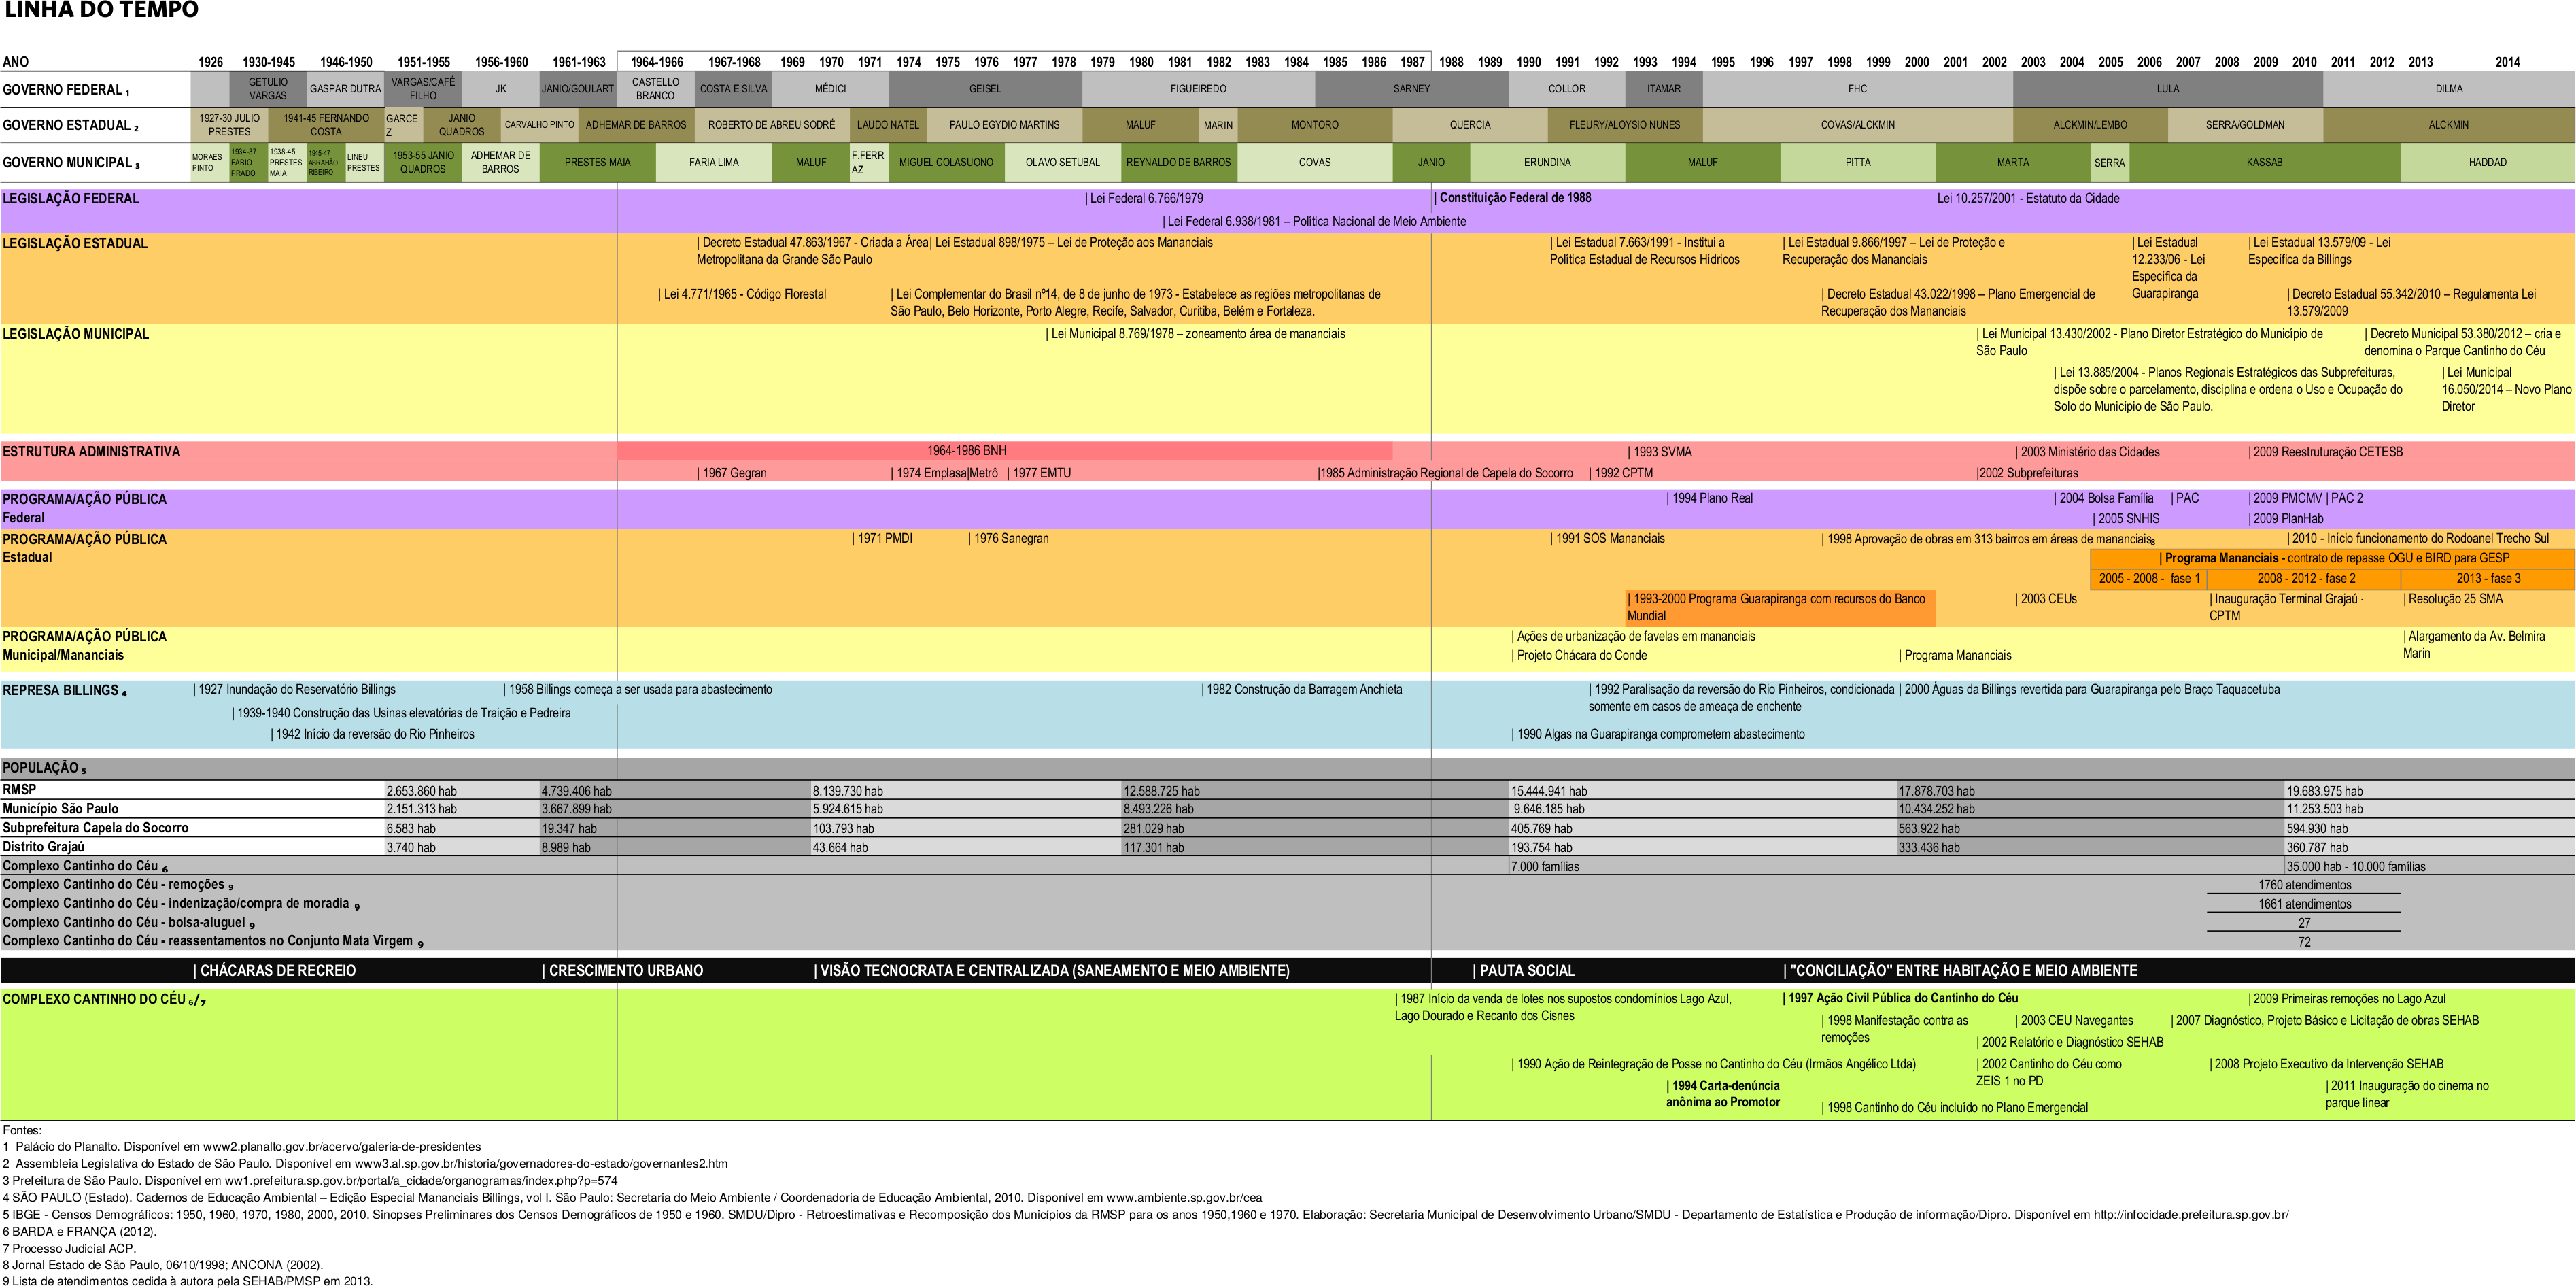
\includegraphics[height=12.6cm,keepaspectratio]{img/matsunaga_linha}
			\label{fig:matsunaga_linha}
			\legend{Fonte: \citeonline[p.39]{Matsunaga2015}}
		\end{figure}
	\end{landscape}
	
	\chapter{Situação atual} \label{hoje}
	
	Para \citeonline[115]{Silva2016}, ``esse parque evidencia uma das maiores contradições que ainda não foram resolvidas pelas políticas públicas: a preservação do meio ambiente e a questão das habitações nesses lugares''. De fato, é inegável que a população ali residente tem elevada proximidade das águas do reservatório, o que cria uma delicada relação entre o meio-ambiente e a interferência antrópica. Ainda conforme \citeonline[p.114]{Silva2016}, a implantação do parque linear foi realizada em parte da orla da península, algo citado pela moradora que realizou o acompanhamento durante a visita de campo (ver seção \ref{visita}).
	
	\begin{citacao}
	    ``A construção do parque linear prevê que ele seja feito em toda a orla da Península do Ribeirão Cocaia, e por enquanto foi feito uma parte de apenas 1,5 km da orla da Península. A política possui a ideia de desfazimento, que é um conceito que a prefeitura do município de São Paulo vinha aplicando durante a gestão Kassab, que previa entre outras coisas a remoção de pessoas que encontravam-se próximos à borda da represa (\dots)''
    \end{citacao}
    
    A assimetria devido à descontinuidade na implantação do parque linear também foi apontada por \citeonline[p.102]{Silva2016}, que realizou visita de campo e esteve em contato com Josiane, que identificou como líder comunitária:
    
    \begin{citacao}
		Já no Cantinho do Céu, o bairro se divide nitidamente na metade da rua
	    Francisco Lopes Solano, onde foram feitas obras de infraestrutura para receber o parque linear que chegaria ao Cantinho do Céu, mas que, segundo seus moradores, foi feito no Lago Azul, não tendo chegado na área onde realmente está localizado o Cantinho do Céu.
    \end{citacao}
    
    Ou seja, podemos concluir que a maior parte do bairro não foi contemplada com áreas de infraestrutura. O projeto não deixa de ser louvável do ponto de vista arquitetônico, muito menos pelos desafios encontrados na compatibilização de diferentes elementos da maquinaria do Estado ----- conforme \citeonline[p.121]{Barda2012} ``a preparação e a execução do Programa Mananciais são de responsabilidade dos três níveis de governo, contando com a participação da comunidade e de outros agentes da sociedade civil'' -----, no entanto, trata-se de uma falha a ser observada, visto que o projeto não foi completamente implantado.
	
	\section{Visita de campo} \label{visita}
	
	A visita de campo foi realizada no período vespertino, em 14/07/2018. A visita foi viabilizada pela Anetilde, professora municipal da rede pública de ensino, conhecida por Gigi, que por sua vez é diretora da rede pública de ensino e está lotada numa escola do distrito, além de ser irmã do meio de Maria, que é namorada de Caio César, um dos integrantes do grupo responsável por este relatório. Coincidentemente, exceto por Caio César, todos os atores são habitantes de longa data da Zona Sul e suas vidas foram ou continuam sendo marcadas pelo contato com o multifacetado distrito do Grajaú.
	
	Para realizar a visita, Caio César se dirigiu à Estação Tatuapé (linhas ) utilizando a linha de ônibus 3763-10 e realizou o trajeto entre ela e a Estação Autódromo utilizando as linhas 11, 4 e 9 do sistema metroferroviário. A partir da Estação Autódromo da \gls{cptm}, o trajeto foi feito com o carro da Gigi, que se dirigiu até a residência de Anetilde. A partir dali, fomos recebidos por Anetilde, seus filhos em idade infantil (um menino e duas meninas gêmeas), sua mãe e seu marido. Anetilde, Gigi, Maria e Caio percorreram então toda a extensão do Parque Linear Cantinho do Céu. Foram realizadas conversas entre Caio e Anetilde, de maneira a melhor compreender a região do Lago Azul e do Parque Residencial dos Lagos, bem como o Cantinho do Céu, além disso, foram capturadas centenas de fotografias do percurso, para posterior referência.
	
	Durante a visita de campo evidenciou-se o apontamento feito por \citeonline[p.94]{Silva2016} acerca da área conhecida pela população como Cantinho do Céu, fronteiriça à área conhecida pela população como Lago Azul, correspondente ao parque linear:
	
	\begin{citacao}
		``Um dos lugares que está crescendo novamente é uma área diante do parque linear, onde já havia sido removida a população, dentro da borda da represa, com habitações recém-construídas, que apresentam um alto grau de precariedade, com a falta de água encanada, de esgoto, e até de fossa asséptica.''
	\end{citacao}
	
	\citeonline[p.96]{Silva2016} salienta que ``essa ocupação está tomando características de perenidade com formação de casas de alvenaria'', o que também se confirmou. Trata-se, inclusive, de um trecho fronteiriço à urbanização no qual não mais é possível enxergar as águas, vide figura \ref{fig:borda_critica}.
	
	\begin{figure}[htb]
		\centering
		\caption[Lago Azul e Cantinho do Céu em 14/07/2018]{Observando o Cantinho do Céu a partir de trecho parcialmente construído do Parque Linear Cantinho do Céu, na área conhecida por Lago Azul pela comunidade, 14 de julho de 2018}
		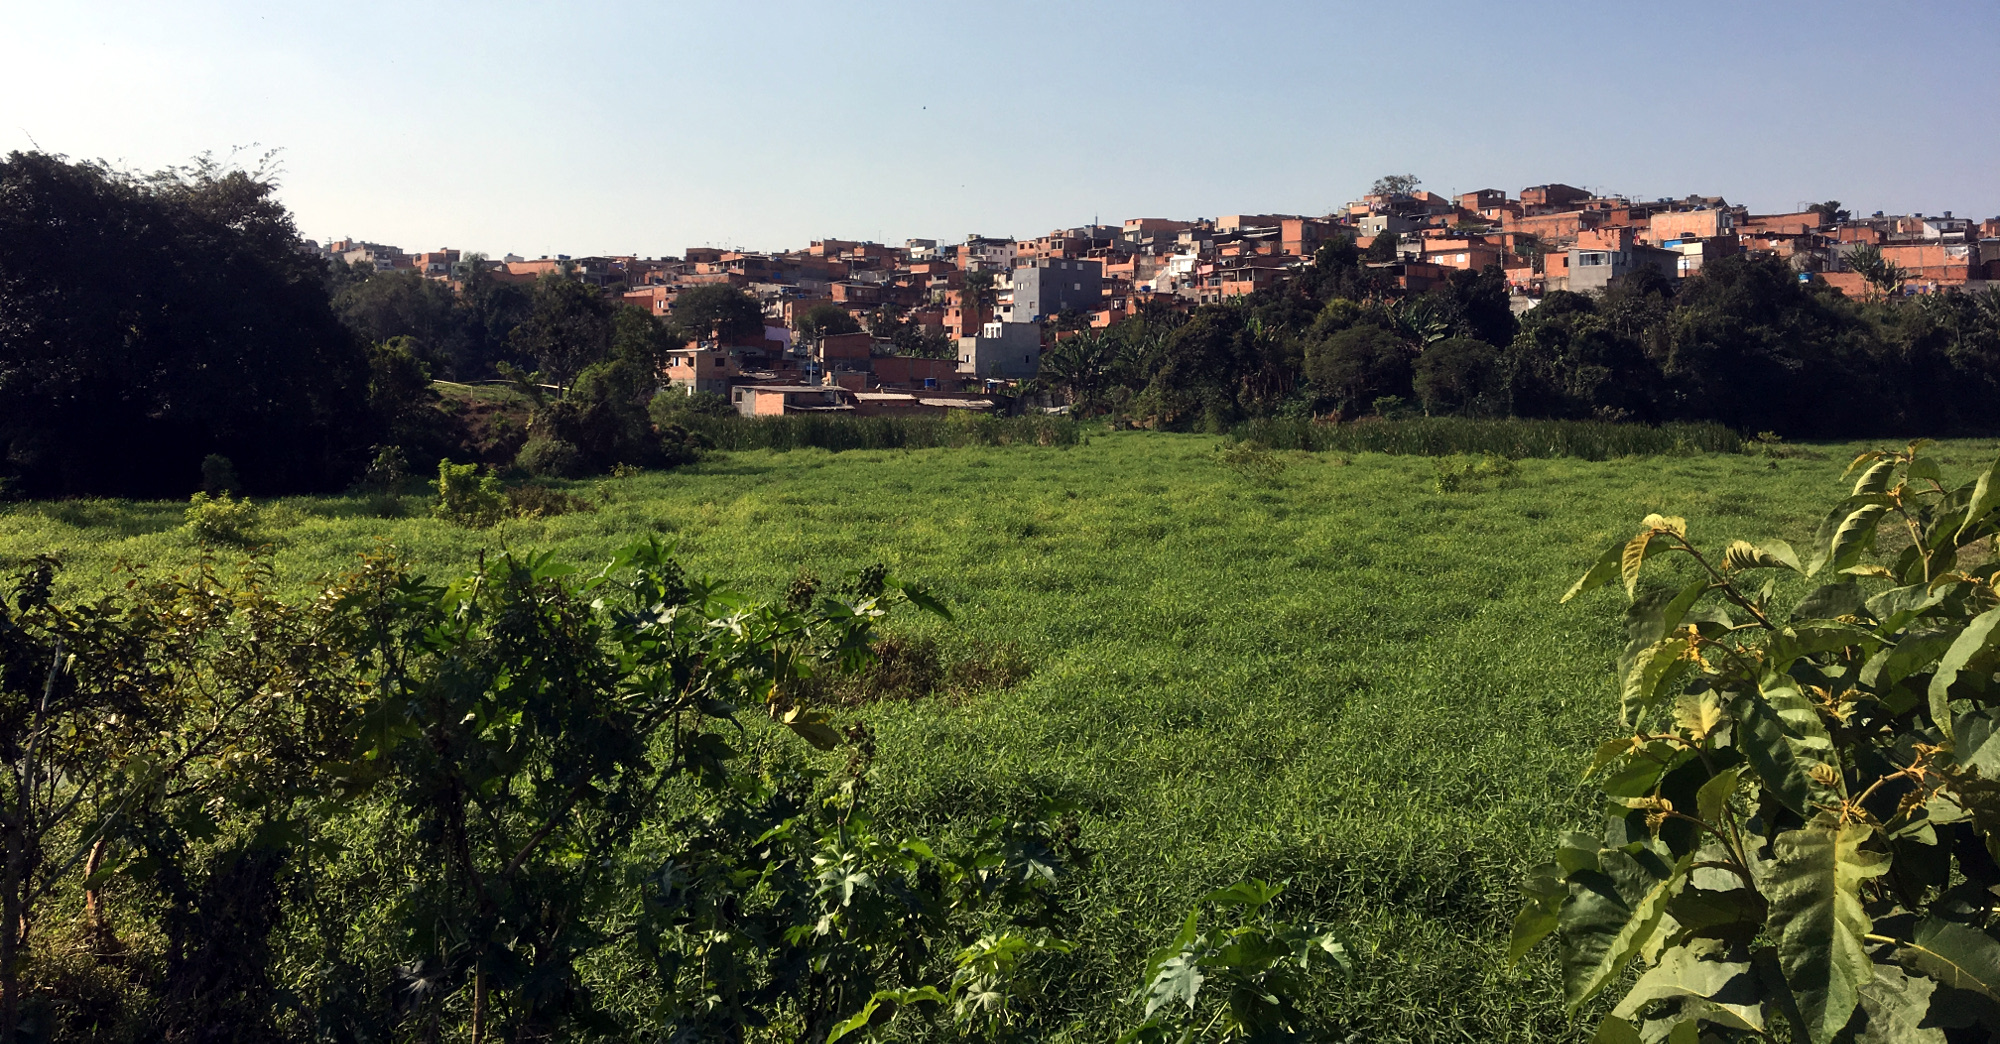
\includegraphics[width=\linewidth]{img/visita_borda_lago_azul_cantinho}
		\label{fig:borda_critica}
		\legend{Elaboração própria}
	\end{figure}
	
	As críticas de \citeonline[p.120]{Silva2016} ligadas ao caráter pontual da intervenção são reiteradas em vista da falta de acompanhamento para a questão habitacional, que é flagrante tanto pelo descontinuidade do próprio parque linear, como pela favela que tem se consolidado como já observava o autor e também foi observado na visita de campo realizada em julho de 2018:
	
	\begin{citacao}
		``O parque linear em si não é o problema, nem tampouco soluciona o problema. No máximo, ele poderia ser parte da solução, uma vez que desapropriar e fazer o parque pode resolver um problema pontual; porém, sem o encaminhamento adequado para a questão habitacional não há como resolver a situação da área de proteção de mananciais.''
	\end{citacao}
	
	Durante a visita de campo evidenciou-se que o parque linear é apropriado pela população, que o utiliza como área de lazer. \citeonline[p.117]{Silva2016} aponta que ``o argumento para remoções está baseado na defesa da água e do meio ambiente de uma maneira geral, além da necessidade de áreas de lazer especialmente nas periferias e para as comunidades carentes'', ao que considera que os argumentos são de grande consistência, mas que também são utilizados para remover populações, mesmo quando há posse da terra, o que agrava o processo de especulação imobiliária inerente ao capitalismo e expulsão dos mais pobres \cite[p.118]{Silva2016}. Durante a visita de campo, Anetilde explica que os moradores do Parque Residencial dos Lagos detinham a posse da terra, ainda que existissem problemas de regularização fundiária ligados ao loteamento em \glsdesc{apm}, sendo assim, aponta que ex-moradores venderam seus imóveis e buscaram realocar-se dentro do Parque Residencial dos Lagos ou ainda dentro do distrito do Grajaú.
	
	%===============================================================================
	%
	
	% ----------------------------------------------------------
	% ----------------------------------------------------------
	\postextual
	
	
	
	% informa o arquivo com a bibliografia. Deve ser o mesmo nome
	% (sem o sufixo) que será informado no ambiente filecontents
	% que está no final deste arquivo. Neste exemplo foi usado 
	% bibitemp.bib e bibtemp. Este comando insere a bibliografia
	% nesta posição (antes dos apêndices, anexos, índice remissivo)
	\bibliography{fontes}
	% ----------------------------------------------------------
	% Glossário
	% ----------------------------------------------------------
	% Consultar manual da classe abntex2 para orientações sobre o
	% uso do glossário.
	\renewcommand{\glossaryname}{Glossário}
	%\renewcommand{\glossarypreamble}{Esta é a descrição do glossário.\\ \\}
	\renewcommand*{\glsseeformat}[3][\seename]{\textit{#1}
		\glsseelist{#2}}
	
	% ---
	% Traduções para o ambiente glossaries
	% ---
	\providetranslation{Glossary}{Glossário}
	\providetranslation{Acronyms}{Siglas}
	\providetranslation{Notation (glossaries)}{Notação}
	\providetranslation{Description (glossaries)}{Descrição}
	\providetranslation{Symbol (glossaries)}{Símbolo}
	\providetranslation{Page List (glossaries)}{Lista de Páginas}
	\providetranslation{Symbols (glossaries)}{Símbolos}
	\providetranslation{Numbers (glossaries)}{Números} 
	% ---
	
	% ---
	% Imprime o glossário
	% ---
	\cleardoublepage
	\phantomsection
	\addcontentsline{toc}{chapter}{\glossaryname}
	% \glossarystyle{index}
	% \glossarystyle{altlisthypergroup}
	\glossarystyle{tree}
	\printglossaries
	% ---
	
	% ----------------------------------------------------------
	% Apêndices
	% ----------------------------------------------------------
	
	% ---
	% Inicia os apêndices. Não esquecer de fechar ao final de
	% todos os apêndices (\end{apendicesenv})
	% ---
	%\begin{apendicesenv}
	
	% Imprime uma página indicando o início dos apêndices
	%\partapendices
	
	% ----------------------------------------------------------
	%\chapter{Primeiro apêndice}
	% ----------------------------------------------------------
	
	%Este é um exemplo de inclusão de capítulos de %apêndice em uma 
	%monografia.  Cada apêndice é tratado como se fosse %um capítulo.
	%Os apêndices devem ser iniciados pelo comando de %ambiente
	%\textbackslash begin\{apendicesenv\} e encerrados %pelo comando 
	%\textbackslash end\{apendicesenv\}.
	
	% ----------------------------------------------------------
	%\chapter{Segundo apêndice}
	% ----------------------------------------------------------
	
	%Este é um exemplo de inclusão de um segundo apêndice. 
	
	%\end{apendicesenv}
	% ---
	
	
	% ----------------------------------------------------------
	% Anexos
	% ----------------------------------------------------------
	
	% ---
	% Inicia os anexos
	% ---
	%\begin{anexosenv}
	
	% Imprime uma página indicando o início dos anexos
	%\partanexos
	
	% ---
	%\chapter{Anexo I}
	% ---
	%Os anexos são similares aos apêndices se distinguindo pelo fato
	%que os apêndices são de autoria do autor da monografia e os 
	%anexos não são da autoria do autor da monografia.  Por exemplo,
	%se incluir no trabalho um modelo de um formulário preenchido
	%por alunos participantes de uma pesquisa, este será um apêndice
	%se o formulário foi criado pelo autor da monografia e será um
	%anexo se o formulário tiver sido criado por outros (por exemplo,
	%é um formulário padrão da escola em que o aluno que o preenche
	%estuda).
	%
	%Mesmo que o formulário tenha sido elaborado pela escola, uma
	%reprodução do formulário preenchido por cada aluno na pesquisa
	%será incluído no apêndice pois envolve o trabalho do autor da
	%monografia ao distribuir, coletar e reproduzir as respostas.
	%
	%Este é um exemplo de inclusão de capítulos de anexos em uma 
	%monografia.  Cada anexo é tratado como se fosse um capítulo.
	%Os anexos devem ser iniciados pelo comando de ambiente
	%\textbackslash begin\{anexoenv\} e encerrados pelo comando 
	%\textbackslash end\{anexoenv\}.
	%
	%\end{anexosenv}
	% ---
	%---------------------------------------------------------------------
	%---------------------------------------------------------------------
	
	%\printindex
	
	% Por padrão são incluídas no trabalho somente as referências
	% citadas ao longo do texto. No comando abaixo foram acrescentadas
	% algumas referências não citadas (neste texto servem apenas como
	% exemplos). Não deve ser usado o comando (mais simples) 
	% \nocite{*}, pois este parece não ser compatível com o
	% abntex2cite
	%\nocite{abntex2cite,abntex2wiki,boyer,eves,iezzi,kletenic,
	%        diomara,steinbruch,intusolatex,feynman,shannon,
	%        luisfelipe,turing}
\end{document}
